\NeedsTeXFormat{LaTeX2e}
\documentclass[a4paper,10pt,twoside,openright,DIV=15,BCOR25mm
%,draft
]{scrbook}
\KOMAoptions{DIV=last}


\pagestyle{headings}
\usepackage[ngerman]{babel}

\usepackage{subfigure}

%\usepackage[latin1]{inputenc}
%\usepackage[applemac]{inputenc} % Mac-Nutzer
\usepackage[utf8]{inputenc}
\usepackage[T1]{fontenc}
\renewcommand{\sfdefault}{phv}
\renewcommand{\rmdefault}{phv}
\renewcommand{\ttdefault}{pcr}
\usepackage{graphicx}
\usepackage{verbatim}
\usepackage{tabularx}
\usepackage{url}
\usepackage{color}
\usepackage{amssymb}
\usepackage{amsmath}
\usepackage{setspace}
\usepackage{listings}
\renewcommand{\lstlistingname}{Algorithm}% Listing -> Algorithm
\renewcommand{\lstlistlistingname}{List of \lstlistingname s}% List of Listings -> List of Algorithms
\usepackage{todonotes}
\usepackage{hyperref}
\usepackage{array}
%\usepackage[table]{xcolor}
\usepackage{colortbl}
\usepackage{booktabs}
\usepackage{float}
%\usepackage{svg}


\lstset{language=VHDL,
  showstringspaces=false,
  frame=single,
  numbers=left,
  basicstyle=\ttfamily,
  numberstyle=\tiny}

% hier Namen etc. einsetzen
\newcommand{\fullname}{Heiko~Foschum}
\newcommand{\email}{heiko.foschum@gmx.de}
\newcommand{\titel}{Konzeption und Realisierung  einer \newline Plattform zur Unterstützung  von \newline therapeutischen Übungen  und Aufgaben}
\newcommand{\jahr}{2016}
\newcommand{\matnr}{856456}
\newcommand{\gutachterA}{Prof. Dr. Manfred Reichert}
\newcommand{\gutachterB}{Dr. Rüdiger Pryss}
\newcommand{\betreuer}{Marc Schickler}
% hier richtige Fakultät auswählen
\newcommand{\fakultaet}{Ingenieurwissenschaften\\und Informatik}
%\newcommand{\fakultaet}{Mathematik und\\Wirtschaftswissenschaften}
%\newcommand{\fakultaet}{Naturwissenschaften}
%\newcommand{\fakultaet}{Medizin}
% nun noch unten das Institut einsetzen
\newcommand{\institut}{Institut für Datenbanken und Informationssysteme}

%color in tables
\usepackage{colortbl}
\definecolor{Gray}{rgb}{0.80784, 0.86667, 0.90196} %dunkelblau
\definecolor{Lightgray}{rgb}{0.9176, 0.95, 0.95686} %hellblau
\definecolor{Akzent}{rgb}{0.6627, 0.63529, 0.55294} %akzentfarbe
\setlength{\arrayrulewidth}{0.1pt}

\clubpenalty 10000
\widowpenalty 10000

\setlength{\parindent}{0pt}
\setlength{\parskip}{1.4ex plus 0.35ex minus 0.3ex}

% Tiefe, bis zu der Überschriften in das Inhaltsverzeichnis kommen
\setcounter{tocdepth}{3}

\pdfinfo{
  /Author (\fullname)
  /Title (\titel)
  /Producer     (pdfeTex 3.14159-1.30.6-2.2)
  /Keywords ()
}

\usepackage{hyperref}
\hypersetup{
pdftitle=\titel,
pdfauthor=\fullname,
pdfsubject={Masterarbeit},
pdfproducer={pdfeTex 3.14159-1.30.6-2.2},
colorlinks=false,
pdfborder=0 0 0	% keine Box um die Links!
}

%Trennungsregeln
\hyphenation{Sil-ben-trenn-ung}
\hyphenation{Sprung-se-quenz-en}
\hyphenation{Sprung-se-quenz}
\hyphenation{Ka-nal-mo-del}
\hyphenation{Ka-nal-mo-dels}
\hyphenation{Bit-Sen-de-dau-er}
\hyphenation{Im-ple-men-tie-rung}
\hyphenation{VHDL-Im-ple-men-tie-rung}
\hyphenation{Sen-de-dau-er}
\hyphenation{FH-FSK-Mo-du-la-ti-on}

\begin{document}
\frontmatter


%Einstellung der Farbe von Tabellen
%\rowcolors{1}{green}{pink}
% Titelseite
\thispagestyle{empty}
\begin{addmargin*}[4mm]{-10mm}

\includegraphics[height=1.8cm]{images/unilogo_bild}
\hfill
\includegraphics[height=1.8cm]{images/unilogo_wort}\\[1em]

{\footnotesize
{\bfseries Universität Ulm} \textbar ~89069 Ulm \textbar ~Germany
\hspace*{50mm}\parbox[t]{65mm}{\bfseries Fakultät für\\
\fakultaet\\
% TODO hier Institut anpassen
\mdseries \institut}\\[2cm]

\parbox{140mm}{\bfseries \huge \titel}\\[0.5em]
{\footnotesize Masterarbeit}\\[3em]

{\footnotesize \bfseries Vorgelegt von:}\\
{\footnotesize \fullname\\\email}\\[2em]
%{\footnotesize \bfseries Bearbeitet mit:}\\                     
%{\footnotesize\bearbeitetMit\\\bearbeitetMitEmail}\\[2em]
{\footnotesize \bfseries Gutachter:}\\ 
{\footnotesize\gutachterA\\
\gutachterB}\\[2em]
{\footnotesize \bfseries Betreuer:}\\ 
{\footnotesize\betreuer}\\\\
{\footnotesize\jahr}
}
\end{addmargin*}


% Impressum
\clearpage
\thispagestyle{empty}
{ \small
  \flushleft
  Fassung \today \\\vfill
  \copyright~\jahr~\fullname\\[0.5em]
% Falls keine Lizenz gewünscht wird bitte den folgenden Text entfernen.
% Die Lizenz erlaubt es zu nichtkommerziellen Zwecken die Arbeit zu
% vervielfältigen und Kopien zu machen. Dabei muss aber immer der Autor
% angegeben werden. Eine kommerzielle Verwertung ist für den Autor
% weiter möglich.
%This work is licensed under the Creative Commons Attribution-NonCommercial-ShareAlike 3.0 License. To view a copy of this license, visit http://creativecommons.org/licenses/by-nc-sa/3.0/de/ or send a letter to Creative Commons, 543 Howard Street, 5th Floor, San Francisco, California, 94105, USA. \\
  Satz: PDF-\LaTeXe
}


% ab hier Zeilenabstand 1,4 fach 10pt/14pt
\setstretch{1.4}

\tableofcontents

\mainmatter
\chapter{Einleitung}
Bei der Betreuung von Patienten durch einen Therapeuten, ob nun in der Psycho-, Physiotherapie oder sogar in der Diätassistenz, sind neben der eigentlich \textbf{Therapie / Behandlung} durch den Therapeuten - Übungen und Fragebögen für Zuhause fast immer Bestandteil der Behandlung. Wie in Abbildung \ref{TherapieAblauf} aufgezeigt werden die Aufgaben in der Sitzung besprochen und sollen dann vom Patienten selbstständig und ohne Betreuung bearbeitet werden.

\begin{figure}[H]
	\centering
	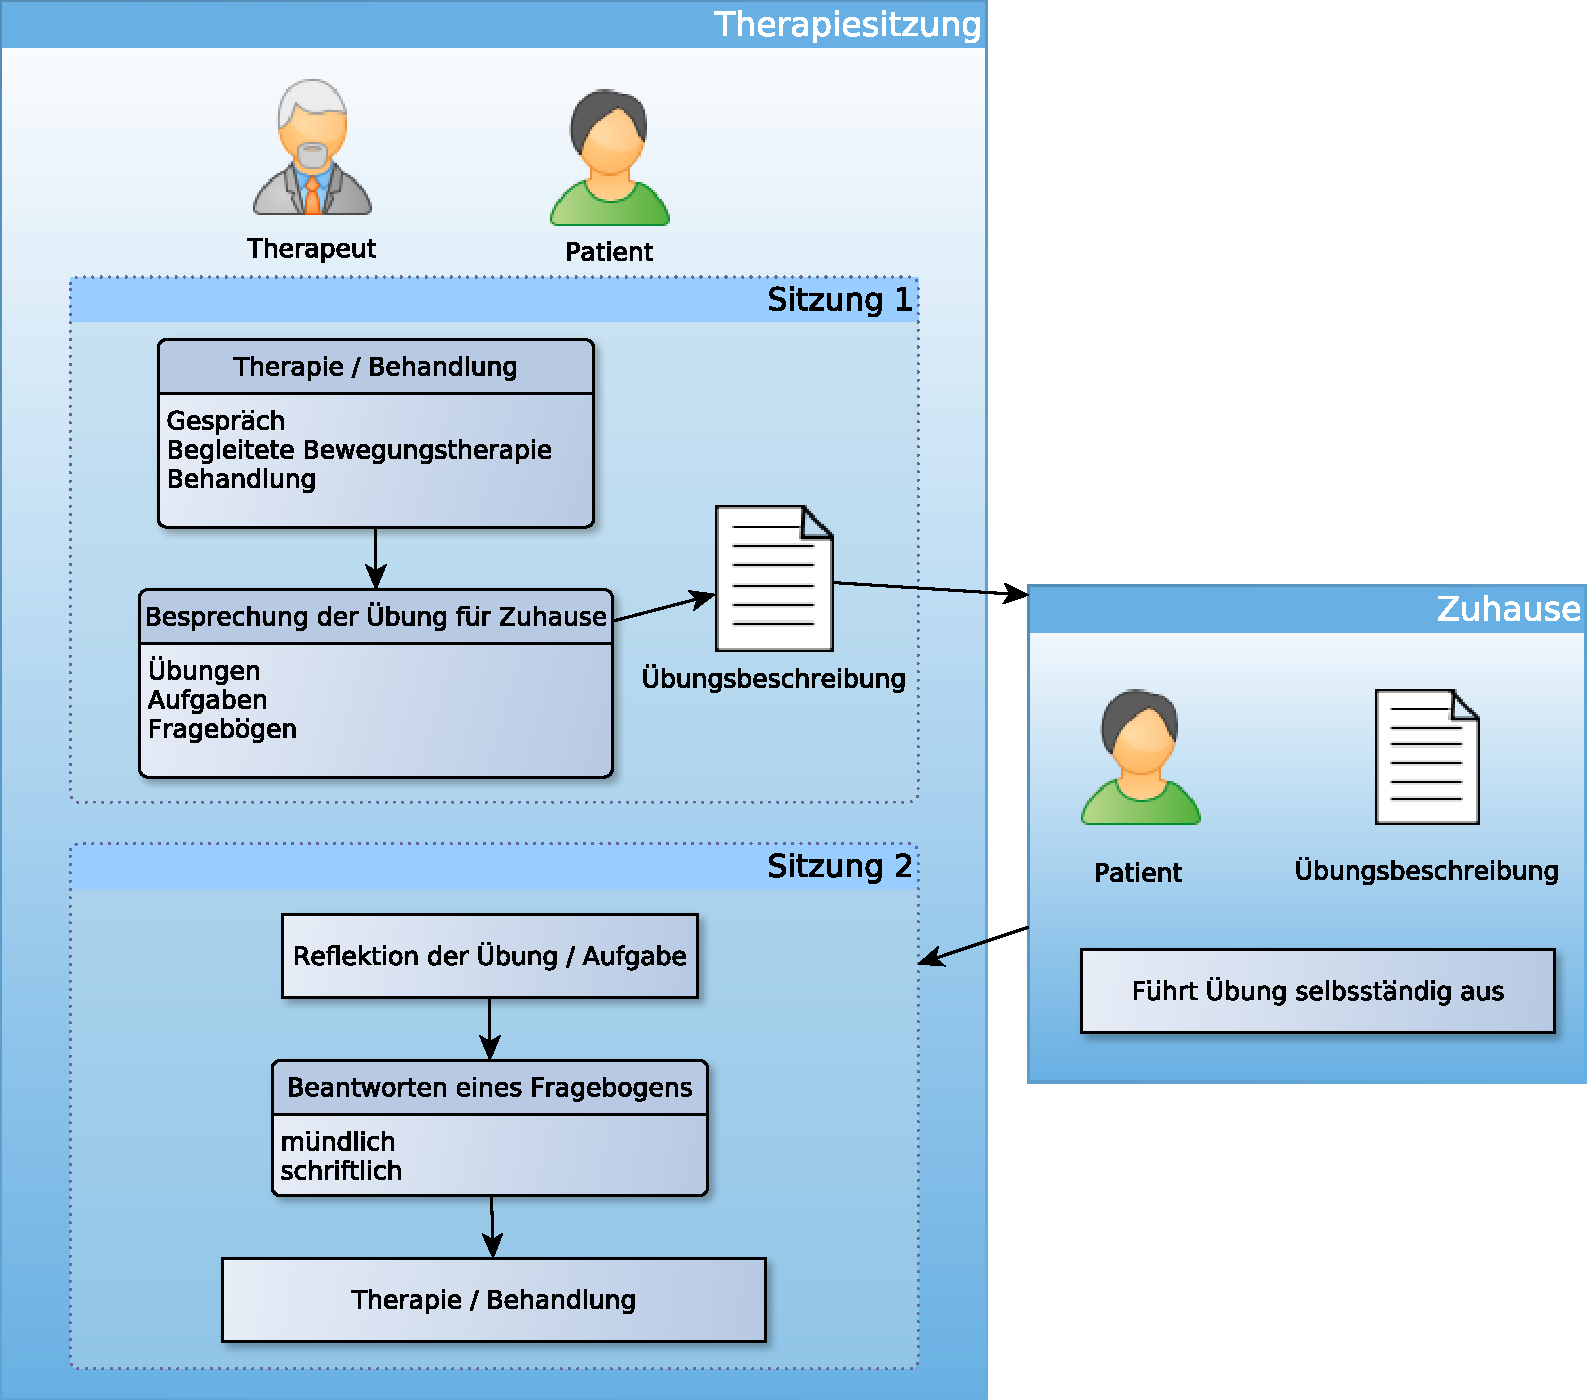
\includegraphics[scale=0.55]{images/TherapieAblauf}
	\caption[Grundlegender Ablauf einer Therapie]{Grundlegender Ablauf einer Therapie}
	\label{TherapieAblauf}
\end{figure}

Diese Aufgaben sind wichtiger Bestandteil für den Behandlungserfolg \cite{SL05}. Sie helfen beim Transfer der Therapie in den Alltag. Jedoch ist eins der größten Probleme bei dieser Vorgehensweise, dass die Aufgaben oft gar nicht oder nur unvollständig erledigt werden \cite{FF01}.

Bisher wurden dieses Aufgaben auf einen Blatt Papier festgehalten und der Patient war selbst dafür Verantwortlich diese in seinen Tagesablauf einzuplanen. Die einzige Vorgabe war es die Aufgabe(n) bis zum nächsten Termin x mal zu machen. Der Therapeut gab im besten Fall lediglich eine Empfehlung wann die Aufgabe zu erledigen ist, nicht jedoch einen genauen Plan an den sich der Patient halten konnte.
\section{Ziel der Arbeit}

Im Zuge dieser Arbeit wurde das Konzept einer Plattform entwickelt und umgesetzt, welches auf der einen Seite dem Patienten hilft sein Aufgabe zu erledigen. Auf der anderen Seite aber auch dem Therapeuten Daten und Feedback zu den Übungen liefert wodurch dieser die Möglichkeit hat den Behandlungserfolg zu steigern.

Auf Grundlage aktueller Software wurde so eine Plattform implementiert, die es dem Therapeuten erlaubt seine Patienten innerhalb einer Webanwendung zu verwalten. Er hat die Möglichkeit, Therapieaufgaben und Fragebögen zu gestalten und diese dem jeweiligen Patienten zuzuordnen.

Anhand einer App wird der Patient sobald das Zeitintervall angefangen hat, daran erinnert seine Aufgabe zu erledigen und zeigt die Aufgabenbeschreibung an. Am Ende des definierten Zeitintervalls hat der Patient die Möglichkeit den zugeordneten Fragebogen auszufüllen. Welcher nach Beendigung wiederum direkt vom Therapeuten eingesehen werden kann.

Ziel ist es vor allem, das die Aufgaben Vollständig und vor allem immer erledigt werden. Aber auch die erzeugte Resonanz und Daten soll zum Therapieerfolg beitragen. Hierdurch können die Therapeutischen Aufgaben verbessert werden und auf den einzelnen Patienten abgestimmt werden.

In einer Studie von Helbig und Fehm \cite{bibid} gaben zwar nur 11\% der befragten an, die Aufgabe nicht erledigt zu haben. Nicht einmal die Hälfte jedoch gaben dagegen an, die Aufgabe genau so wie beschreiben ausgeführt zu haben. Durch das Anzeigen der Aufgabenbeschreibung soll dem Patienten geholfen werden die Aufgabe genau so durchzuführen wie vorgegeben. Durch die angehängten Materialien in jeglicher digitalen Form kann der Patient vielseitig bei seinem persönlichen Erfolg unterstützt werden.

\section{Aufbau der Arbeit}
\todo{Aufbau der Arbeit + Grafik}

 und die Implementierung der Anwendung vorgestellt. Im Entwurf wird die Vision, die Anforderungsanalyse und der daraus resultierende Architekturentwurf aufgezeigt. Darauf folgt eine Software Analyse, welche sich damit auseinander setzt welche Frameworks verwendet werden könnten um die gestellte Aufgabe zu lösen. Anschließend wird im Unterkapitel Implementierung [\ref*{Implementierung}] auf selbige eingegangen. Dies beinhaltet das zugrundeliegende Datenmodell so wie die Erläuterung der Implementierungen des Servers sowie der beiden Clients für Therapeut und Patient.


\chapter{Grundlagen} \label{Theoretische Grundlagen}
Im diesem Kapitel werden die Theoretischen Grundlagen der verwendeten Technologien im einzelnen betrachtet.
\section{(Web)Grundlagen}
REST, HTML(5)(GET,SET,...),Client-Server Architektur, JavaScript, Zentralisierung der Daten (Sicherheit)
\section{Anwendungsentwicklung für mobile Geräte}
Eine der Grundvoraussetzungen dieser Arbeit sollte die Verfügbarkeit auf möglichst vielen Plattformen sein. Auch wenn während dieser Arbeit aus verschiedenen Gründen, die später noch aufgezeigten werden, früh klar war das die Wahl auf den sogenannten MEAN-Stack fällt, werden hier dennoch einige andere Frameworks und Plattformen aufgezeigt. Sowohl für die Desktop Anwendung des Therapeuten, also auch für die mobile Anwendung des Patienten.
\subsection{Möglichkeiten der Anwendungsentwicklung}
Am Anfang jeder mobilen Anwendung steht die Entscheidung auf welchen Geräten diese laufen soll. Zum einen besteht die Möglichkeit eine Anwendung nativ für eine bestimmte Plattform zu entwickeln. Um die App auf anderen Plattformen zu bringen ist es dann jedoch nötig diese praktisch neu zu implementieren. Aus diesem Dilemma heraus entstanden verschiedenen Frameworks die es dem Entwickler möglich machen direkt für mehrere Plattformen zu entwickeln.
\subsubsection{Plattform spezifische Entwicklung}
\paragraph*{Vorteile der nativen Anwendungsentwicklung} %weg und flusstext
\todo{ausformulieren}
Direkter Zugriff auf die Hardware ( Kamera und GPS) 

\subsubsection{Cross Plattform Entwicklung}
Von Cross Plattform Entwicklung spricht man, wenn der Code der entwickelten Anwendung nicht nur für eine spezifische Plattform verwendbar ist. 
Es gibt etlichen Frameworks die es erlauben Code einmal zu schreiben und ihn dann auf verschiedenen Plattformen laufen zu lassen. Dies wird Grundlegend auf \textbf{3 verschiedenen} Wegen erreicht:
\paragraph{Web-Apps / Webanwendungen}laufen im, vom Betriebssystem zur Verfügung gestellten Webbrowser. Hierbei ist das Betriebssystem völlig egal, es werden nur einige Voraussetzungen an den Webbrowser gestellt. Ebenso wird eine aktive Internetverbindung benötigt wenn die App ausschließlich online zur Verfügung steht. Um dies zu umgehen wurde in HTML5 verschiedenen Möglichkeiten eingebaut um Code und Daten lokal zwischenzuspeichern zu können. Dies bietet den Vorteil, dass die App schnell veröffentlicht und aktualisiert werden kann. Wenn der Nutzer mit einer aktiven Internet Verbindung öffnet aktualisiert sich die App automatisch. 
Der Nachteil dadurch das die App im Webbrowser läuft ist, dass man nur zugriff auf die Funktionen hat, die dieser bietet. Da ein Webbrowser nicht zwangsläufig auf einem mobilen Gerät mit diversen Sensoren laufen muss, ist der zugriff auf die gängigen Sensoren in einem mobilen Endgerät meinst sehr eingeschränkt. Auf Grund dessen muss man sich bei der Web-App Entwicklung meist auf Kamera, Datenpersistenz und GPS beschränken. Durch die Zentralisierung der App sieht diese auf jedem Gerät gleich aus. Dies erscheint im ersten Augenblick positiv, der Benutzer jedoch ist an das Bedienkonzept seines Betriebssystems gewohnt.

\todo{inhalt mit reinbringen. link im kommentar}%https://de.wikipedia.org/wiki/Webanwendung#/media/File:Webanwendung_client_server_01.png

\paragraph{Hybride Apps} basieren wie auch die Web-Apps auf den Webtechnologien HTML5, CSS und JavaScript und laufen in einem mitgelieferten Minibrowser(Webview Container).Dieser Container ist in einer nativen App eingebettet was den Zugriff auf die System APIs des Geräts erlaubt. Durch das einbetten von nativen Code ist der Zugriff auf alle vom Betriebssystem zur Verfügung gestellten Funktionen möglich. wie z.b. GPS, Kamera, Betriebssystem Benachrichtigungen und die verschiedenen Sensoren(Beschleunigung, Umgebungslicht, Hall, Gyroskop,...). 
Da die Anwendung im Herzen eine Internetseite ist, ist es implizit möglich diese unter einer URL zu veröffentlichen und wie eine Web-App zu behandeln. Dann jedoch auch mit den Einschränkungen die diese bietet. Für den Entwickler sehr angenehm sind oft angebotene "Live-View" Technologien. Diese erlauben durch speichern einer HTML oder JavaScript Projektdatei ein neu laden der App im Webbrowser zu initiieren. Dies bietet ein schnelles Designen der Oberfläche und implementieren grundlegender Funktionen. Systemeigene Funktionen müssen jedoch auf einem Gerät oder im Emulator getestet werden. Hierzu ist jedoch compilieren, packen und das ausliefern notwendig, was etwas Zeit genötigt.

\todo{Wikipediaartikel is nochmal anders beschrieben} %https://de.wikipedia.org/wiki/Mobile_App#Hybrid-Apps


\subsection{Desktop}
Angular, Qt, ...
\subsection{Mobile Anwendung}
PhoneGap + Ionic[1 und 2 ] %http://ionicframework.com/docs/overview/#cordova
		 What the ionic framework provides is the native look and feel and the user interface interactions

Xamarin  

 (http://thinkapps.com/blog/development/develop-for-ios-v-android-cross-platform-tools/) 




\chapter{Entwurf}\label{Entwurf} 
Im folgenden Kapitel wird der Entwurf der Plattform vorgestellt. Dies beinhaltet die Vision, welche aufzeigt was von der zu entwickelten Anwendung erwartet wird und welche Arbeitsabläufe von ihr abgedeckt werden sollen.
In der darauf folgenden Anforderungsanalyse [\ref{Anforderungsanalyse}] wird sich damit auseinandergesetzt, welche Einzelteile zur Realisierung der Plattform benötigt werden und welche Anforderungen an diese gestellt werden. 

\section{Vision}\label{Vision}
Mit Hilfe der zu entwickelnden Plattform soll es möglich sein Therapieaufgaben / Übungen und Fragebögen im Zuge einer therapeutischen Betreuung zwischen Therapeut und Patient auf digitalem Weg auszutauschen. Hierdurch soll das in Kapitel 1 erwähnte Blatt Papier auf welchem die Aufgabe oder Übung beschrieben ist wegfallen und durch eine zeitgemäße App für das mobile Endgeräte des Patienten ersetzt werden.

\begin{figure}[H]
	\centering
	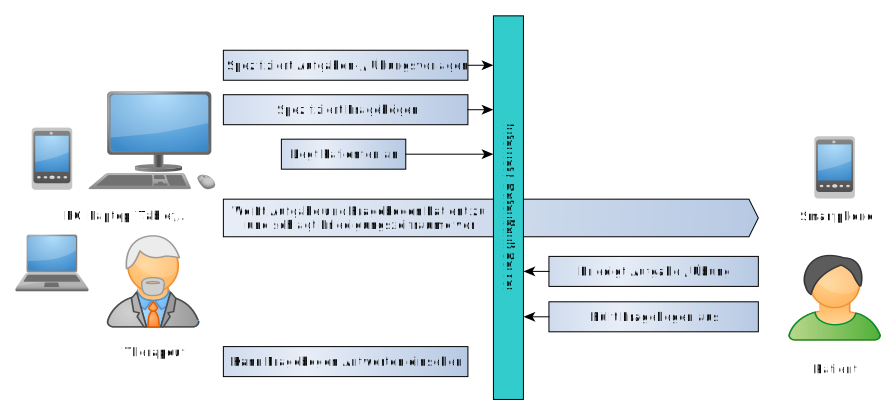
\includegraphics[scale=0.6]{images/AblaufAbstrakt}
	\caption[Workflow Diagramm vom erstellen der Aufgabe/Übung inc. Fragebogen bis zur Erledigung/Beantwortung]{Workflow Diagramm vom erstellen der Aufgabe/Übung inc. Fragebogen bis zur Erledigung/Beantwortung}
	\label{AblaufAbstrakt}
\end{figure}

Dies gibt dem Therapeuten auch die Möglichkeit, digitale Medien zur Veranschaulichung der Aufgabe / Übung zu verwenden, welche der Patient während er die Aufgabe oder Übung macht vorliegen hat. Wodurch diesem die korrekte Durchführung der Aufgabe erleichtert wird.

Hierdurch wird es auch möglich völlig neue Aufgaben und Übungen zu konzipieren. Dem Patienten könnten auf diesem Weg auch Medien wie etwa Bilder oder Videos mit nach Hause gegeben werden. Denkbar wäre auch interaktive Medien wie Spiele oder ähnliches.

Der Therapeut möchte in einer Desktop Anwendung seine Patienten verwalten können, sowie Vorlagen für therapeutische Aufgaben, Übungen und Fragebögen erstellen. Um diese dann den einzelnen Patienten zuweisen zu können. Ebenso soll es für den Therapeuten möglich sein Fragebögen mit von den Antworten abhängigen Fragen zu erstellen um diese nach erfolgreicher Erledigung der therapeutischen Aufgabe oder Übung von den Patienten beantworten zu lassen.

Um möglichst viele Patienten mit dieser Plattform unterstützen zu können, soll diese für möglichst viele Smartphone Betriebssysteme implementiert werden. Die wichtigsten sind hierbei Android, iOS und WindowsPhone.

Die Mobile App des Patienten soll dann auf das Profil des Patienten, welches durch den Therapeuten angelegt wurde, zugreifen. Hierbei werden die Daten über die zugewiesenen Aufgaben und Fragebögen abgerufen.

Zu den vom Therapeut vorgegebenen Zeiten werden dann Betriebssystem Erinnerungen erstellt. Welche den Patienten an das erledigen der Aufgabe erinnern. Die vorgegebene Zeitspanne soll vom Patienten verändert werden können. Hierdurch soll der Anteil der Patienten welche ihre Aufgabe gar nicht erledigen verringert werden.

Nach vollenden der Aufgabe oder am Ende der gegebenen Zeitspanne soll der Patient die Möglichkeit haben den zugehörigen Fragebogen auszufüllen.
\section{Anforderungsanalyse}\label{Anforderungsanalyse}
Um eine gemeinsame Datenbasis zu schaffen muss es einen im Internet erreichbaren Server geben. Dieser hält die vom Therapeuten eingegebene Daten. Dies erreicht man durch einen beliebigen persistenten Speicher, wie beispielsweise eine Datenbank oder ein Dateisystem. Der Server bietet hierbei eine Webschnittstelle zur Datenbank an, über welche sowohl der Therapeuten Client als auch die mobile Anwendung Zugriff auf die Daten hat. 

\paragraph{Der Therapeuten Client} soll dem Therapeuten die Oberfläche bieten mit Hilfe welcher es ihm möglich sein muss die Patienten, Therapieaufgaben / Übungen und Fragebögen verwalten zu können. Die Patienten müssen angelegt, angezeigt, bearbeitet und gelöscht werden können.

Des weiteren muss es dem Therapeuten möglich sein, Aufgaben zu spezifizieren, diese sollen neben Name und Beschreibung auch verschieden Medien beinhalten können. Der Therapeut soll außerdem die Möglichkeit haben Kontrollmechanismen an die Aufgabe anzuhängen, welche ihm Feedback darüber geben ob und wie der Patient die Aufgabe erledigt hat, damit dieser sich nicht nur auf das mündliche Feedback des Patienten verlassen muss.

In der Anzeige eines Patienten soll der Therapeut die zuvor erstellten Therapieaufgaben / Übungsvorlagen sowie Fragebögen diesem zuweisen können. Bei der Zuweisung gibt der Therapeut das/die Ereignisse(Zeit, Ort, etc.) an zu denen der Patient an die Aufgabe erinnert werden soll.

Ebenso muss der Therapeuten Client einen Mechanismus bieten in welchem der Therapeut Fragebögen erstellen kann, in welchen die nächste Frage von der Antwort der zuvor gestellten Frage abhängig ist.

Nachdem ein Fragebogen von einem Patienten beantwortet wurde muss es dem Therapeuten möglich sein, diesen einzusehen.



\paragraph{Der Patienten Client} soll auf möglichst vielen mobilen Plattformen lauffähig sein, damit so wenig Patienten wie möglich von dieser neuen Methode der Therapeut - Patient Interaktion ausgeschlossen werden.

Der Patient muss nach dem ersten Start der mobilen Anwendung Verbindung zu seinem Profil herstellen können, etwa durch Eingabe eines Benutzernamens oder einer ID. Dieser Vorgang sollte durch einen Sicherheitsmechanismus geschützt werden, um die Daten des Patienten vor dem Zugriff Unbefugter zu schützen.

Anschließend müssen die Daten zu den hinterlegten Therapieaufgaben über die Webschnittstelle des Servers geladen und weiterverarbeitet werden. Die Ereignisse zu den Aufgaben werden in so weit verarbeitet, dass der Patient an die Therapieaufgabe erinnert wird, wenn das Startereignis der Aufgabe eingetreten ist. Die mobile Anwendung soll die Möglichkeit bieten, die vom Therapeuten vorgegebenen Ereignisse anzupassen.

Ist das Startereignis eingetroffen, soll der Patienten Client eine Ansicht bieten, in welcher dieser die Details zu der anstehenden Aufgabe / Übung einsehen kann. Des weiteren muss er die Möglichkeit haben, die angehängten Materialien auf möglichst einfache Weiße einzusehen um das erledigen der Aufgabe / Übung so einfach wie es nur geht zu gestalten. Je weniger Hindernisse der Patient hierbei hat, desto höher ist die Chance, dass dieser die Aufgabe auch wirklich macht. Was wiederum den Therapieerfolg erhöht. Die Detailansicht zu einer bestimmten Aufgaben sollte jederzeit aufrufbar sein, nicht nur wenn das Startereignis eingetroffen ist.

Der Client für den Patienten sollte ebenso die Option bieten, eine Übersicht über alle zugewiesenen Aufgaben anzuzeigen. 

\newpage
\subsection{Funktionale Anforderungen}
Aus der Vision [Kapitel \ref{Vision}] und der Anforderungsanalyse [Kapitel \ref{Anforderungsanalyse}] können folgende funktionale Anforderungen für die beiden Clients abgeleitet werden.

\subsubsection{Datenbank Server}
Für den Datenbank Server können die in Tabelle \ref{FunktionaleAnforderungenServer} aufgezeigten funktionalen Anforderungen spezifiziert werden.
\begin{table} [H]
	\begin{center}
		\begin{tabular}{p{0,5cm} p{4cm} p{10cm}}
			\rowcolor{black!20} \textbf{Nr.} & \textbf{Anforderung} & \textbf{Beschreibung} \\
			\hline \toprule
			1.1 & \textbf{Datenpersistenz} & Die empfangenen Daten müssen persistent gespeichert werden \\ \hline \addlinespace
			1.2 & \textbf{Daten Sicherung} & Automatische Sicherung der Daten auf Zweitsystem \\ \hline \addlinespace
			1.3 & \textbf{Datenschnittstelle} & Schnittstelle für den Datenaustausch mit unterschiedlichen Geräten \\ \hline \addlinespace
		\end{tabular}
	\end{center}
	\label{FunktionaleAnforderungenServer}
	\caption[Funktionale Anforderungen an den Datenbank Server]{Funktionale Anforderungen  an den Datenbank Server}
\end{table}

\subsubsection{Therapeuten Client}
Für den Client des Therapeuten sind dies die in Tabelle \ref{TabelleFunktionaleAnforderungenTherapeutClient} dargestellten Anforderungen.

\begin{table}[htbp]
	\begin{center}
		\begin{tabular}{p{1cm} p{4cm} p{9,5cm}}
			\rowcolor{black!20}\textbf{Nr.} & \textbf{Bezeichnung} & \textbf{Beschreibung} \\ \toprule 
			\rowcolor{black!5}2.1 & \textbf{Patientenverwaltung} & Die Patienten sollen mit ihren persönlichen Daten angezeigt und verwaltet werden können \\ \hline \addlinespace
			2.1.1 & anlegen & Einen neuen Patienten hinzufügen \\ \hline \addlinespace
			2.1.2 & editieren & Einen bestehenden editieren \\ \hline \addlinespace
			2.1.3 & löschen & Einen bestehenden löschen \\ \hline \addlinespace
			\rowcolor{black!5}2.2 & \textbf{Aufgabenverwaltung} & Verwaltung und Anzeige von Aufgaben / Übungsvorlagen \\ \hline \addlinespace
			2.2.1 & anlegen & Eine neue Vorlage hinzufügen \\ \hline \addlinespace
			2.2.2 & editieren & Einen bestehenden editieren \\ \hline \addlinespace
			2.2.3 & löschen & Eine bestehenden löschen \\ \hline \addlinespace
			\rowcolor{black!5}2.3 & \textbf{Fragebogenverwaltung} & Verwaltung und Anzeige von Fragebögen \\ \hline \addlinespace
			2.3.1 & anlegen & Eine neue Vorlage hinzufügen \\ \hline \addlinespace 
			2.3.2 & editieren & Einen bestehenden editieren \\ \hline \addlinespace
			2.3.3 & löschen & Eine bestehenden löschen \\ \hline
		\end{tabular}
	\end{center}
	\caption[Anforderungen an den Therapeuten Client]{Anforderungen an den Therapeuten Client}
	\label{TabelleFunktionaleAnforderungenTherapeutClient}	
\end{table}

\newpage
\subsubsection{Aufgaben-/Übungsvorlagen}
Dabei sollen die Aufgaben/Übungen mittels der in Tabelle \ref{TabelleFunktionaleAnforderungenAufgaben} aufgezeigten Daten spezifiziert werden können.

\begin{table}[htbp]
	\begin{center}
		\begin{tabular}{p{0,5cm} p{4cm} p{10cm}}
			\rowcolor{black!20} \textbf{Nr.} & \textbf{Bezeichnung} & \textbf{Beschreibung} \\ \toprule 
			A.1 & \textbf{Name} & Ein kurzer, aussagekräftiger Name der Aufgaben-/Übungsvorlage \\ \hline \addlinespace
			A.2 & \textbf{Beschreibung} & Die textuelle Beschreibung der Aufgabe/Übung in beliebiger Länge \\ \hline \addlinespace
			A.3 & \textbf{Materialien} & Die Möglichkeit beliebig viele, unterschiedliche Materialien anzuhängen \\ \hline \addlinespace
			A.4 & \textbf{Kontrollmechanismen} & Spezifikation von Kontrollmechanismen welche Rückmeldung darüber geben ob die Aufgabe erledigt worden ist \\ \hline \addlinespace
			A.5 & \textbf{Kategorisierung} & Mechanismus um die Aufgaben/Übungen in Kategorien einordnen zu können um die Übersichtlichkeit zu erhöhen  \\ \hline \addlinespace
			A.6 & \textbf{Verschiedene Erledigungskontexte} & Verschiedene Wege um zu spezifizieren wann der Patient an die Aufgabe erinnert werden soll \\ \hline \addlinespace
		\end{tabular}
	\end{center}
	\caption[Anforderungen an die Vorlage einer Aufgabe/Übung]{Anforderungen an die Vorlage einer Aufgabe/Übung}
	\label{TabelleFunktionaleAnforderungenAufgaben}
\end{table}

\subsubsection{Fragebögen}
Die Anforderungen an die Fragebogenerstellung werden in der Tabelle \ref{TabelleFunktionaleAnforderungenFragebogen} aufgezeigt.

\begin{table}[htbp]
	\begin{center}
		\begin{tabular}{p{0,5cm} p{4cm} p{10cm}}
			\rowcolor{black!20} \textbf{Nr.} & \textbf{Bezeichnung} & \textbf{Beschreibung} \\ \toprule 
			B.1 & \textbf{Name} & Ein kurzer, aussagekräftiger Name um den Fragebogen identifizieren zu können \\ \hline \addlinespace
			B.2 & \textbf{Beschreibung} & Für eine textuelle Beschreibung des Fragebogens \\ \hline \addlinespace
			B.3 & \textbf{Antwortabhängige Fragen} & Möglichkeit um nächste Frage von der gegebenen Antwort des Patienten abhängig zu machen \\ \hline \addlinespace
			B.4 & \textbf{Verschiedene Fragetypen} & Option bieten um unterschiedliche Fragetypen stellen und beantworten zu können  \\ \hline \addlinespace
		\end{tabular}
	\end{center}
	\caption[Anforderungen an die Fragebogen Erstellung]{Anforderungen an die Fragebogenerstellung}
	\label{TabelleFunktionaleAnforderungenFragebogen}
\end{table}

Durch vier unterschiedliche Fragetypen können in der Regel alle Arten von Fragen abgebildet werden. Diese Typen werden in der Tabelle \ref{TabelleFunktionaleAnforderungenFragebogenTypen} aufgezeigt und näher spezifiziert.

\begin{table}[H]
	\begin{center}
		\begin{tabular}{p{0,5cm} p{4cm} p{10cm}}
			\rowcolor{black!20} \textbf{Nr.} & \textbf{Fragetyp} & \textbf{Beschreibung} \\ \toprule 
			C.1 & \textbf{Einzelantwort} & Aus mehreren Antwortmöglichkeiten kann \textbf{genau eine} ausgewählt werden \\ \hline \addlinespace
			C.2 & \textbf{Mehrfachantwort} & Aus mehreren Antwortmöglichkeiten können \textbf{beliebig viele} aus gewählt werden \\ \hline \addlinespace
			C.3 & \textbf{Bewertung} & Zu den einzelnen Fragen können \textbf{numerische Bewertungen} in einen definierten Bereich abgegeben werden  \\ \hline \addlinespace
			C.4 & \textbf{Freitext} & Die Frage wird durch einen \textbf{freien Text} beantwortet  \\ \hline \addlinespace
		\end{tabular}
	\end{center}
	\caption[Übersicht über die benötigten Fragetypen]{Übersicht über die benötigten Fragetypen}
	\label{TabelleFunktionaleAnforderungenFragebogenTypen}
\end{table}

\subsubsection{Patienten Client}
Für den Client des Patienten sind dies die in Tabelle \ref{FunktionaleAnforderungenPatientClient} dargestellten Anforderungen.

\begin{table}[htbp]
	\begin{center}
		\begin{tabular}{p{0,5cm} p{4cm} p{10cm}}
			\rowcolor{black!20} \textbf{Nr.} & \textbf{Anforderung} & \textbf{Beschreibung} \\	\toprule
			3.1 & \textbf{User Identifikation} & Der Patient stellt Verbindung zu dem von Therapeut erstellten Profil her \\ \hline \addlinespace
			3.2 & \textbf{Aufgabenanzeige} & Übersicht der zugewiesenen therapeutischen Aufgaben \\ \hline \addlinespace
			3.3 & \textbf{Detailanzeige der Aufgabe}  & Eine detaillierte Anzeige der Aufgabe mit Name, Erklärung und angefügten Materialien\\ \hline \addlinespace
			3.4 & \textbf{Anzeige der Materialien} & Die angehängten Materialien müssen vom Patienten innerhalb des Clients eingesehen werden können\\ \hline \addlinespace
			3.5 & \textbf{Verändern des Erledigungskontext} & Der von Therapeuten vorgegebene Erledigungskontext soll vom Patienten veränderbar sein \\ \hline \addlinespace
			3.6 & \textbf{Erinnerung} & Der Patient soll an die Aufgabe erinnert werden \\ \hline \addlinespace
			3.7 & \textbf{Fragebogen beantworten} & Es muss möglich sein, einen Fragebogen zu beantworten \\ \hline \addlinespace
		\end{tabular}
	\end{center}
	\caption[Funktionale Anforderungen an den Patienten Client]{Funktionale Anforderungen an den Patienten Client}
	\label{FunktionaleAnforderungenPatientClient}
\end{table} 
\newpage
\subsection{Nicht-Funktionale Anforderungen}
Aus der Vision [\ref{Vision}] und der Anforderungsanalyse [\ref*{Anforderungsanalyse}] können folgende Nicht-Funktionale Anforderungen sowohl für den Datenbank Server als auch für die beiden Clients abgeleitet werden. 


\subsubsection{Datenbank Server}
Für den Datenbank Server können die in Tabelle \ref{NichtFunktionaleAnforderungenServer} aufgezeigten Anforderungen abgeleitet werden.
\begin{table} [H]
	\begin{center}
		\begin{tabular}{p{0,5cm} p{4cm} p{10cm}}
			\rowcolor{black!20} \textbf{Nr.} & \textbf{Anforderung} & \textbf{Beschreibung} \\
			\hline \toprule
			4.1 & \textbf{kurze Reaktionszeiten} & Der Server sollte möglichst geringe Reaktionszeiten haben \\ \hline \addlinespace
			4.2 & \textbf{Sicherheit} & Die Daten sind vor dem Zugriff Unbefugter zu schützen \\ \hline \addlinespace
		\end{tabular}
	\end{center}
	\label{NichtFunktionaleAnforderungenServer}
	\caption[Nicht-Funktionale Anforderungen an den Server]{Nicht-Funktionale Anforderungen an den Server}
\end{table}

\subsubsection{Therapeuten / Patienten Client}
Für die beiden Clients gelten die in Tabelle \ref{NichtFunktionaleAnforderungenClients} beschriebenen Anforderungen.
\begin{table} [H]
	\begin{center}
		\begin{tabular}{p{0,5cm} p{4cm} p{10cm}}
		\rowcolor{black!20} \textbf{Nr.} & \textbf{Anforderung} & \textbf{Beschreibung} \\
		\hline \toprule
		5.1 &\textbf{ Natives Design} & Die Anwendung soll auf jedem Gerät das gewohnte Design haben um die Usability zu erhöhen \\ \hline \addlinespace
		5.2 & \textbf{vertretbare Reaktionszeiten} & Keine unzumutbaren Wartezeiten \\ \hline \addlinespace
		5.3 & \textbf{einfache Bedienung} & Die Anwendung zielt auf eine möglichst einfach Bedienung ab welche keine Fachkenntnisse benötigt \\ \hline \addlinespace
		\end{tabular}
	\end{center}
	\label{NichtFunktionaleAnforderungenClients}
	\caption[Nicht-Funktionale Anforderungen an die Clients]{Nicht-Funktionale Anforderungen an die Clients}
\end{table}



%%%%%%%%%%%%%%%%%%%%%%%%%%%%%%%%%%%%%%%%%%%%%%%%%%%%%%%%%%%%%%%%%%%%%%%%%%%%%%%%%%%%%%%%%%%%%%%%%%%%%%%%%%%%%%%%%%%%%%%%%%%%%%%%%%%%%%%%%%%%%%%%
%%%%%%%%%%%%%%%%%%%%%%%%%%%%%%%%%%%%%%%%%%%%%%%%%%%%%%%%%%%%%%%%%%%%%%%%%%%%%%%%%%%%%%%%%%%%%%%%%%%%%%%%%%%%%%%%%%%%%%%%%%%%%%%%%%%%%%%%%%%%%%%%
%%%%%%%%%%%%%%%%%%%%%%%%%%%%%%%%%%%%%%%%%%%%%%%%%%%%%%%%%%%%%%%%%%%%%%%%%%%%%%%%%%%%%%%%%%%%%%%%%%%%%%%%%%%%%%%%%%%%%%%%%%%%%%%%%%%%%%%%%%%%%%%%
%%%%%%%%%%%%%%%%%%%%%%%%%%%%%%%%%%%%%%%%%%%%%%%%%%%%%%%%%%%%%%%%%%%%%%%%%%%%%%%%%%%%%%%%%%%%%%%%%%%%%%%%%%%%%%%%%%%%%%%%%%%%%%%%%%%%%%%%%%%%%%%%
%%%%%%%%%%%%%%%%%%%%%%%%%%%%%%%%%%%%%%%%%%%%%%%%%%%%%%%%%%%%%%%%%%%%%%%%%%%%%%%%%%%%%%%%%%%%%%%%%%%%%%%%%%%%%%%%%%%%%%%%%%%%%%%%%%%%%%%%%%%%%%%%

\chapter{Implementierung}\label{_Implementierung}
In diesem Kapitel wird auf die Implementierung der Anwendung eingegangen. Dies beinhaltet den Architekturentwurf, das zugrundeliegende Datenmodell, sowie die Implementierungen des Servers und der beiden Clients für Therapeut und Patient.

Um eine gemeinsame Datenbasis zwischen Therapeuten Client und Patienten App zu schaffen wurde eine \textbf{Datenbank Server} aufgesetzt. Dieser beinhaltet eine Verbindung zu einer MongoDB \textbf{Datenbank}.
\begin{figure}[H]
	\centering
	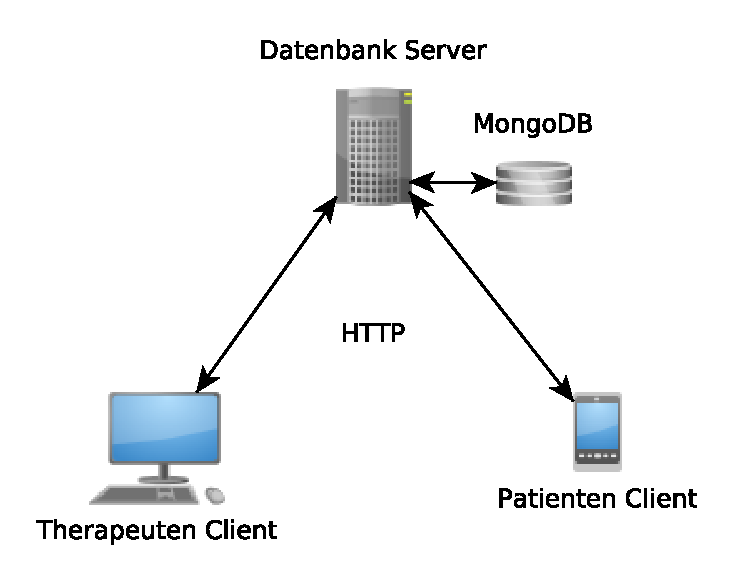
\includegraphics[scale=1.0]{images/ClientServerArchitektur}
	\caption[Client-Server Architektur der Plattform]{Client-Server Architektur der Plattform}
	\label{ClientServerArchitektur}
\end{figure}
Des weiteren wurde eine \textbf{Webserver} implementiert welcher eine \textbf{Web API} anbietet. Dieser fungiert als Bindeglied zwischen Internet und der Datenbank. Er implementiert die HTTP Methoden \textbf{GET, PUT, POST und DELETE}. Hierdurch können von überall auf der Welt die auf dem Server gespeicherten Daten zu Patienten,Therapieaufgaben und Fragebögen abgerufen, verändert oder gelöscht werden.

Als weiterer Baustein für die Plattform wurde eine Client für den Therapeuten auf Basis einer Webseite implementiert. Der Vorteil einer Website besteht darin, dass es völlig egal is welches Betriebssystem der Therapeut verwendet. Es wird lediglich ein Webbrowser und eine aktive Internetverbindung benötigt. Änderungen die an den Patientendaten vorgenommen werden, werden direkt auf dem Datenbank Server gespeichert. Der Client selbst hält dabei keine Daten, außer die temporären, welche zur Anzeige benötigt werden.

Für den Patienten wurde eine \textbf{Cross-Plattform-App} entwickelt, welche sich die benötigten Daten ebenso von dem oben erwähnten Datenbank Server lädt. Die App basiert auf den Technologien \textbf{AngularJS, Cordova und Ionic}. Durch sie wird der Patient mittels einer Betriebssystem Erinnerung an seine Therapeutische Aufgabe erinnert wenn das Start Event eingetroffen ist. Durch Klick auf die Erinnerung wird dem Patient die Aufgabenbeschreibung angezeigt. Wodurch ihm die korrekte Ausführung der Aufgabe erleichtert werden soll.

Durch die Verwendung von \textbf{AngularJS} für den Therapeuten Client wurde erreicht, dass beide mittels JavaScript und HTML5 implementiert werden können.
\newpage
\section{Datenmodell} \label{_Datenmodell}
Um eine einheitliche Datenstruktur auf den beiden Clients und dem Server zu behalten, wurde das folgende Datenmodell entworfen.


Auf Grundlage des \textbf{Datenmodells} [Abbildung \ref*{Datenmodell}] können alle innerhalb der Anwendung benötigten Daten in der Datenbank gespeichert werden.
Jede Datenstruktur beinhaltet eine global einzigartige \textbf{ID}. Diese stellt sicher das die Objekte in der Datenbank wieder gefunden werden kann.
Allen voran möchte der Therapeut seine Patienten verwalten können. Hierzu wurde eine Klasse \textbf{Patient} angelegt. Diese beinhaltet neben der ID, Felder für den Namen, die Adresse und andere Personenbezogene Daten, die in erster Linie dazu verwendet werden, um den Patienten eindeutig zu Identifizieren.
Des weiteren beinhaltet diese Klasse ein Array in dem die zugeordneten Therapieaufgaben gespeichert werden können. Somit is es dem Therapeuten möglich den angelegten Patienten beliebig viele Therapieaufgaben zuzuordnen. 

\begin{figure}[H]
	\centering
	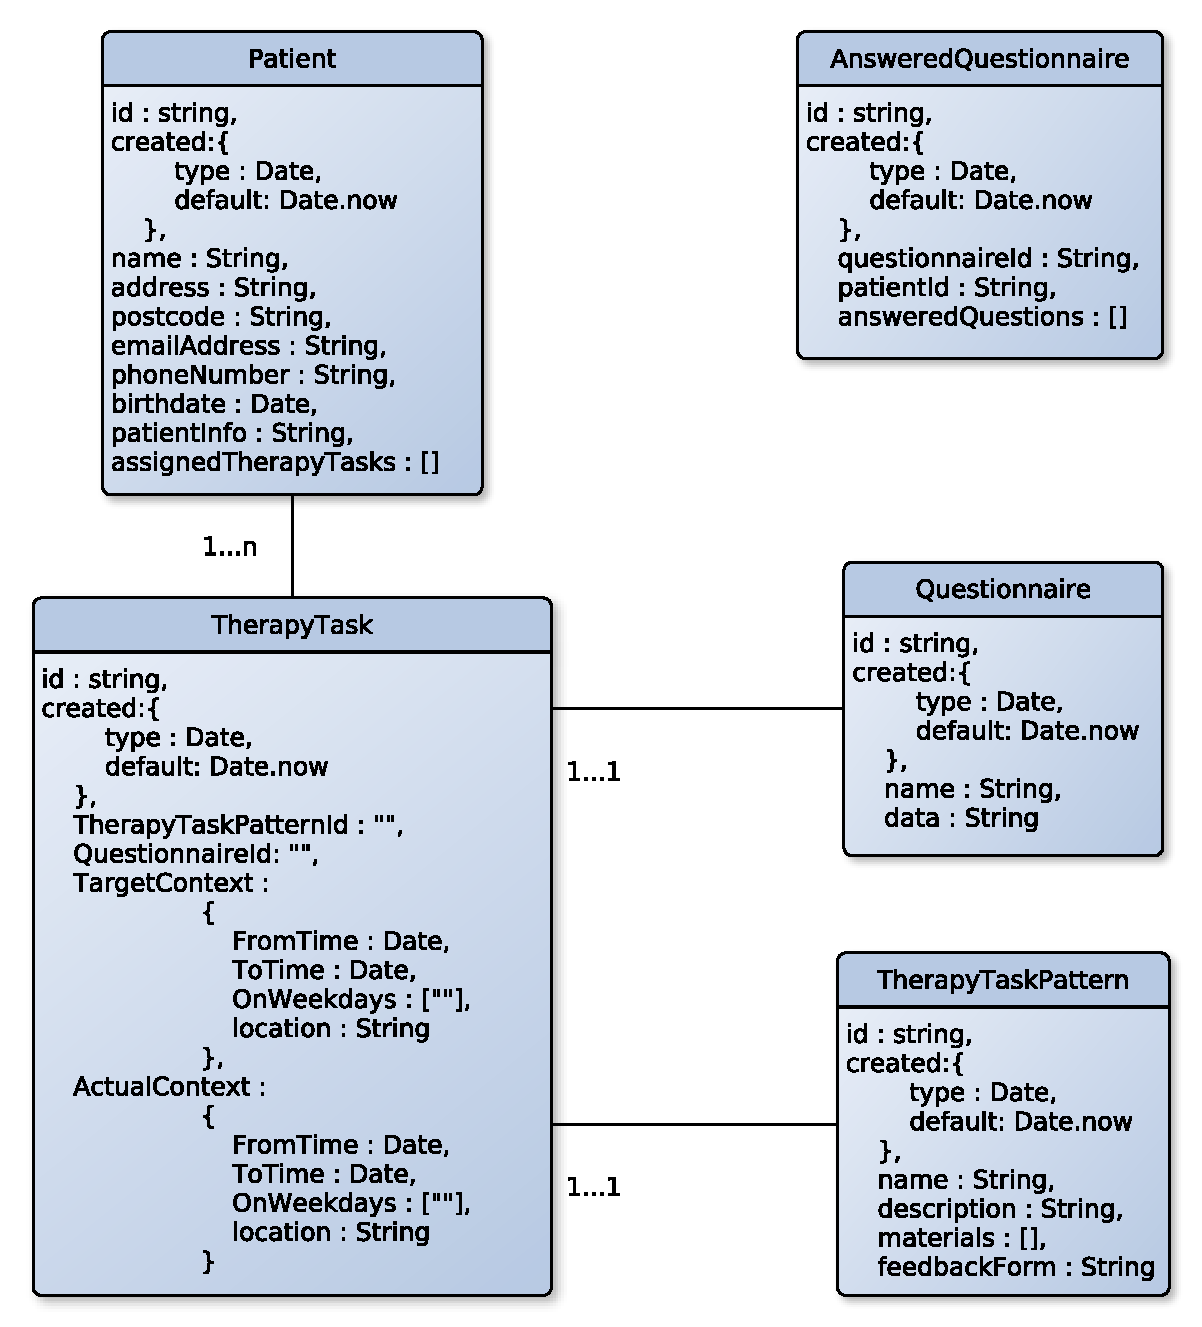
\includegraphics[scale=0.6]{images/datenModell}
	\caption[Visualisierung des Datenmodells]{Visualisierung des Datenmodells}
	\label{Datenmodell}
\end{figure}

Diese Informationen werden in der Klasse \textbf{TherapyTask} gespeichert. Diese ist zwar immer Bestandteil der Klasse Patient, wurde aber zur besseren Abgrenzung von dieser separiert.
TherapyTask beinhaltet jeweils ein Feld für die ID eines Fragebogens sowie die ID einer Aufgabenvorlage. Hierdurch ist es möglich die Daten des zugehörigen, vom Therapeut ausgewählten, Fragebogen und die der Aufgabe vom Server zu laden und im Client anzuzeigen.

Die vom Therapeuten vorgegebenen Zeitintervalle oder Orte zu/an denen die Aufgabe erledigt werden sollte können unter dem Eintrag \textbf{TargetContext} gespeichert werden. Zum Abschluss der Arbeit besteht dieser Kontext aus der \textbf{FromTime}, welche den Start der zeitlichen Erledigungszeitintervalls beschreibt und der \textbf{ToTime} welche das Ende des Intervalls angibt. In dem Array \textbf{OnWeekdays} werden die Wochentage gespeichert an denen die Übung zu erledigen ist. Der Variable \textbf{location} soll in Zukunft dazu verwendet werden können um das Startevent nicht nur Zeit sonder auch Ortsabhängig definieren zu können.
Unter dem Eintrag \textbf{ActualContext} können die vom Patienten veränderten Erledigungsdaten gespeichert werden.

Die erstellten Fragebögen werden in der Klasse \textbf{Questionnaire} gespeichert. Diese beinhaltet neben einem Feld für den Namen des Fragebogens ein weiteres um die vom Fragebogendesigner  erstellten Daten im XML Format als String zu speichern.
Die Klasse \textbf{TherapyTaskPattern} wird verwendet um die Vorlagen für Therapieaufgaben zu speichern. Diese beinhaltet neben dem Namen und der Beschreibung der Aufgabe ein Array, in welchem angehängte Materialien gespeichert werden können. Dies können jegliche Art von Zeichenfolgen sein, werden aber bisher nur verwendet um Internetadressen zu speichern, da sich hinter diesen theoretisch jede Information verbergen kann.

\newpage
\subsection{Datenbank Server} \label{_ImpDatenbankServer}
Zur Implementierung des in Kapitel \ref{Anforderungsanalyse} angesprochenen Webservers wurde \textbf{NodeJS} \cite{NODE16} als Basis verwendet. Dies bietet eine JavaScript Laufzeitumgebung. Mittels des Package-Managers \textbf{npm} wurde dann das Web-Framework \textbf{express} \cite{EXP16} installiert. Durch dieses Framework bietet eine grundlegende Implementierung eines Webservers. Dieser bietet einen lauffähigen HTTP Server sowie eine Grundlegende Implementierung eines sogenannten Routers und einem Webfrontend. Um eine spätere Trennung von REST-API und Therapeuten Client einfach zu machen sind diese voneinander getrennt. Hierzu wurden aus dem Express-Starter-Projekt alle Abhängigkeiten entfernt die zur Darstellung einer Website benötigt werden. 

\begin{figure}[H]
	\centering
	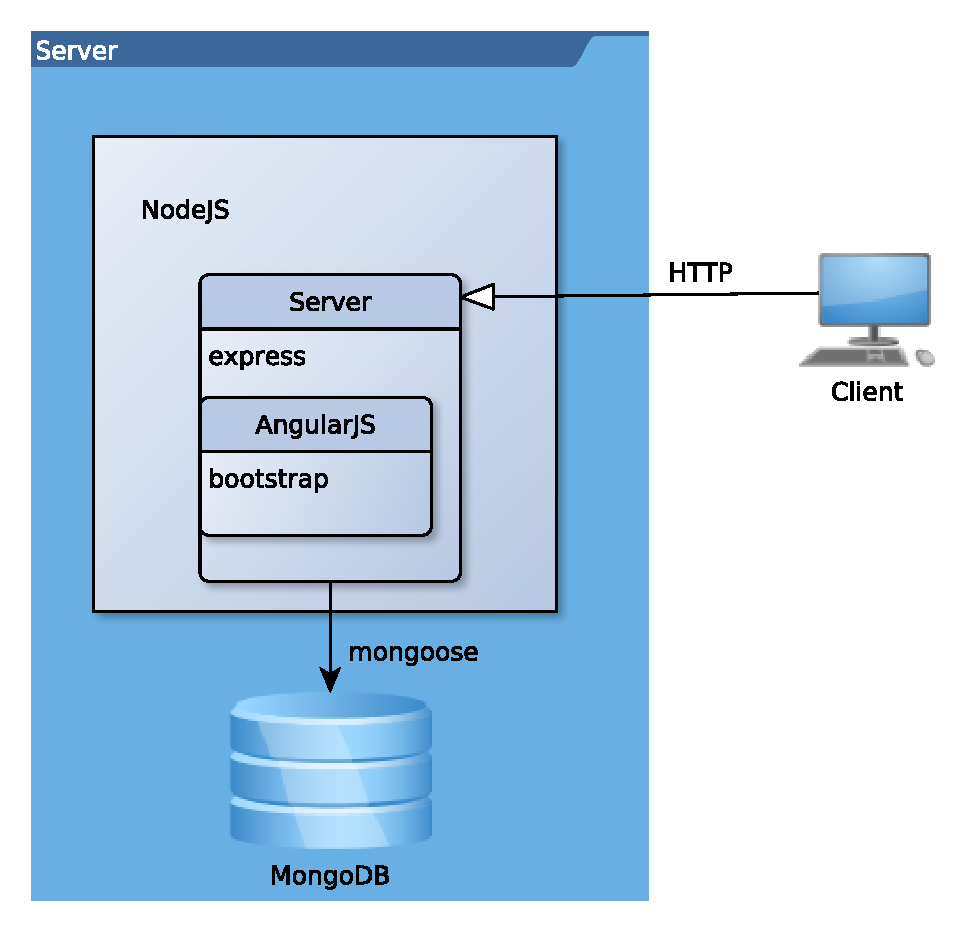
\includegraphics[scale=0.7]{images/ServerArchitektur}
	\caption[Übersicht über die Architektur des Servers]{Übersicht über die Architektur des Servers}
	\label{ServerArchitektur}
\end{figure}

Wie in der \textbf{package.json} unter \textbf{scripts} -> \textbf{start}\ angegeben wird beim Start des Servers durch \textbf{npm start} die Datei www.js ausgeführt. Diese Startet mittels des \textbf{http} Moduls einen Webserver welcher auf den angegebene Port horcht. Zusätzlich wird durch einen \textbf{require} die server.js eingebunden in welcher der Server weiter spezifiziert ist. In dieser Datei wird express eingebunden und gestartet. Unter Verwendung des \textbf{mongoose} Moduls wird die Verbindung zur Datenbank durch \textbf{mongoose.connect('mongodb://localhost/patient')} hergestellt. Diese muss vorher auf dem System installiert und gestartet werden.
\begin{figure}[H]
	\centering
	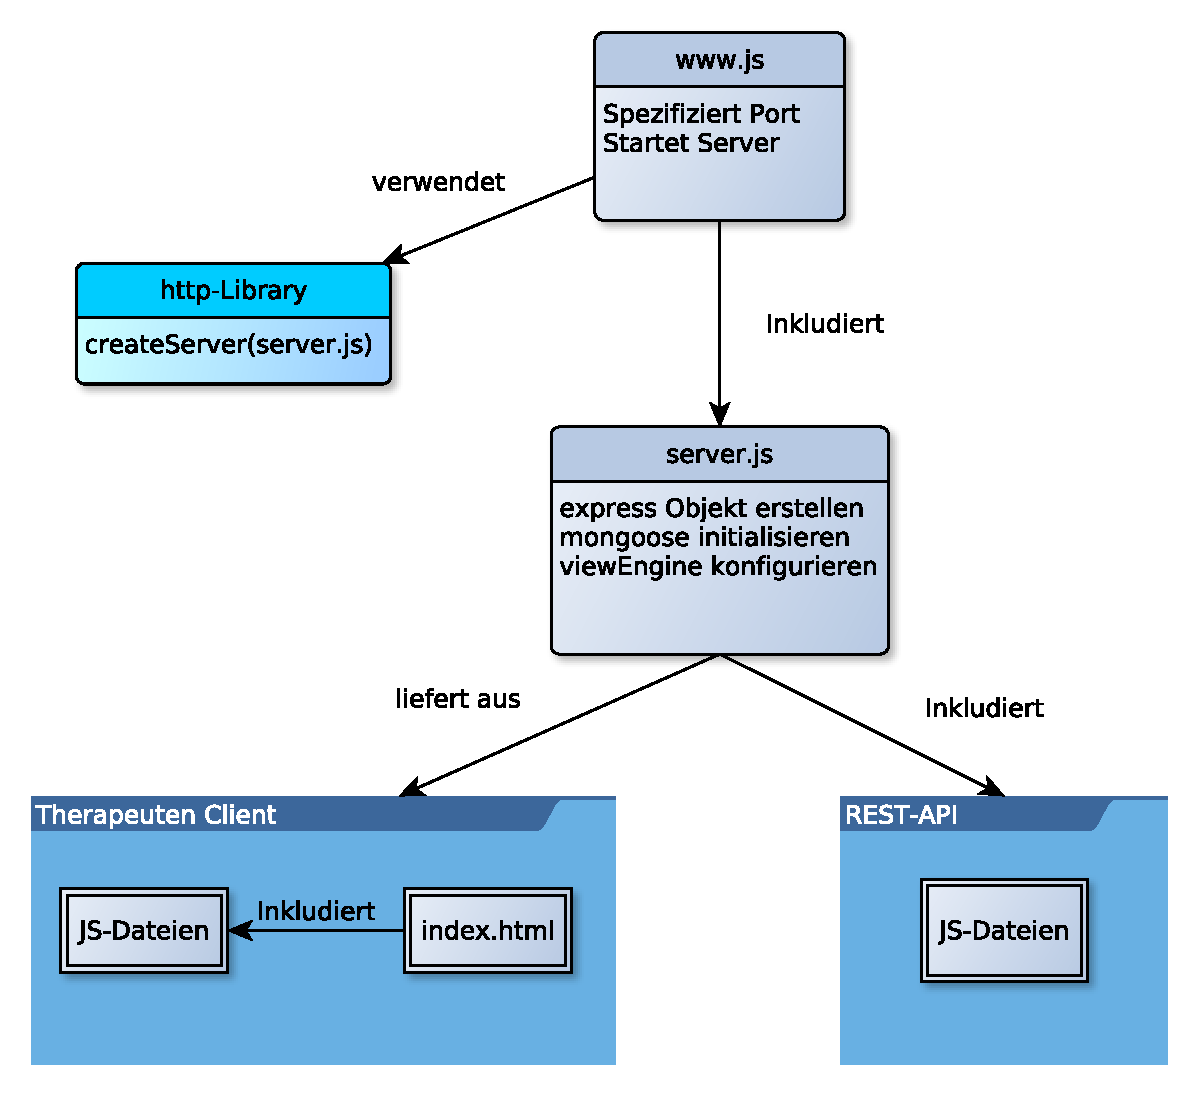
\includegraphics[scale=0.6]{images/ServerScriptArchitektur}
	\caption[Script Architektur des Servers]{Script Architektur des Servers}
	\label{ServerScriptArchitektur}
\end{figure}
Anhand des eingebauten Routers können durch unterschiedlicher URLs bestimmte Programmteile auszuführen. Mittels \textbf{express.use('/patientAPI',patient)} wurde eine Universelle Route für die Patienten-API erstellt. Diese leitet die HTTP Anfrage an die hinter \textbf{patient} spezifizierte Datei (patientsAPI.js) weiter. Hier werden die Routen der Patienten API näher spezifiziert wie in Abbildung \ref{REST Architektur} veranschaulicht.

Zur Umsetzung der API wurden diesem Router unterschiedliche URL-Pfade mittels \\ \textbf{router.get('/:patientId', patients.show);} bekannt gemacht. Durch hinzufügen dieser Route wird der Server unter seiner gewohnten Adresse + \textbf{/:patientId} die Antwort der Funktion \\ \textbf{patients.show()} zurückgeben. Diese Route wird fortan für alle GET Anfragen in Form von \\ /patientAPI/"<beliebigerString"> verwendet. Der Zusatz :patientId gibt an, dass die angehängte Daten innerhalb von patients.show() unter der Variable PatientId abgerufen werden kann. Innerhalb von patients.show() wird dann mittels \textbf{req.params.patientId} die ID des angefragten Patientenobjekts ausgelesen.
 \begin{figure}[H]
 	\centering
 	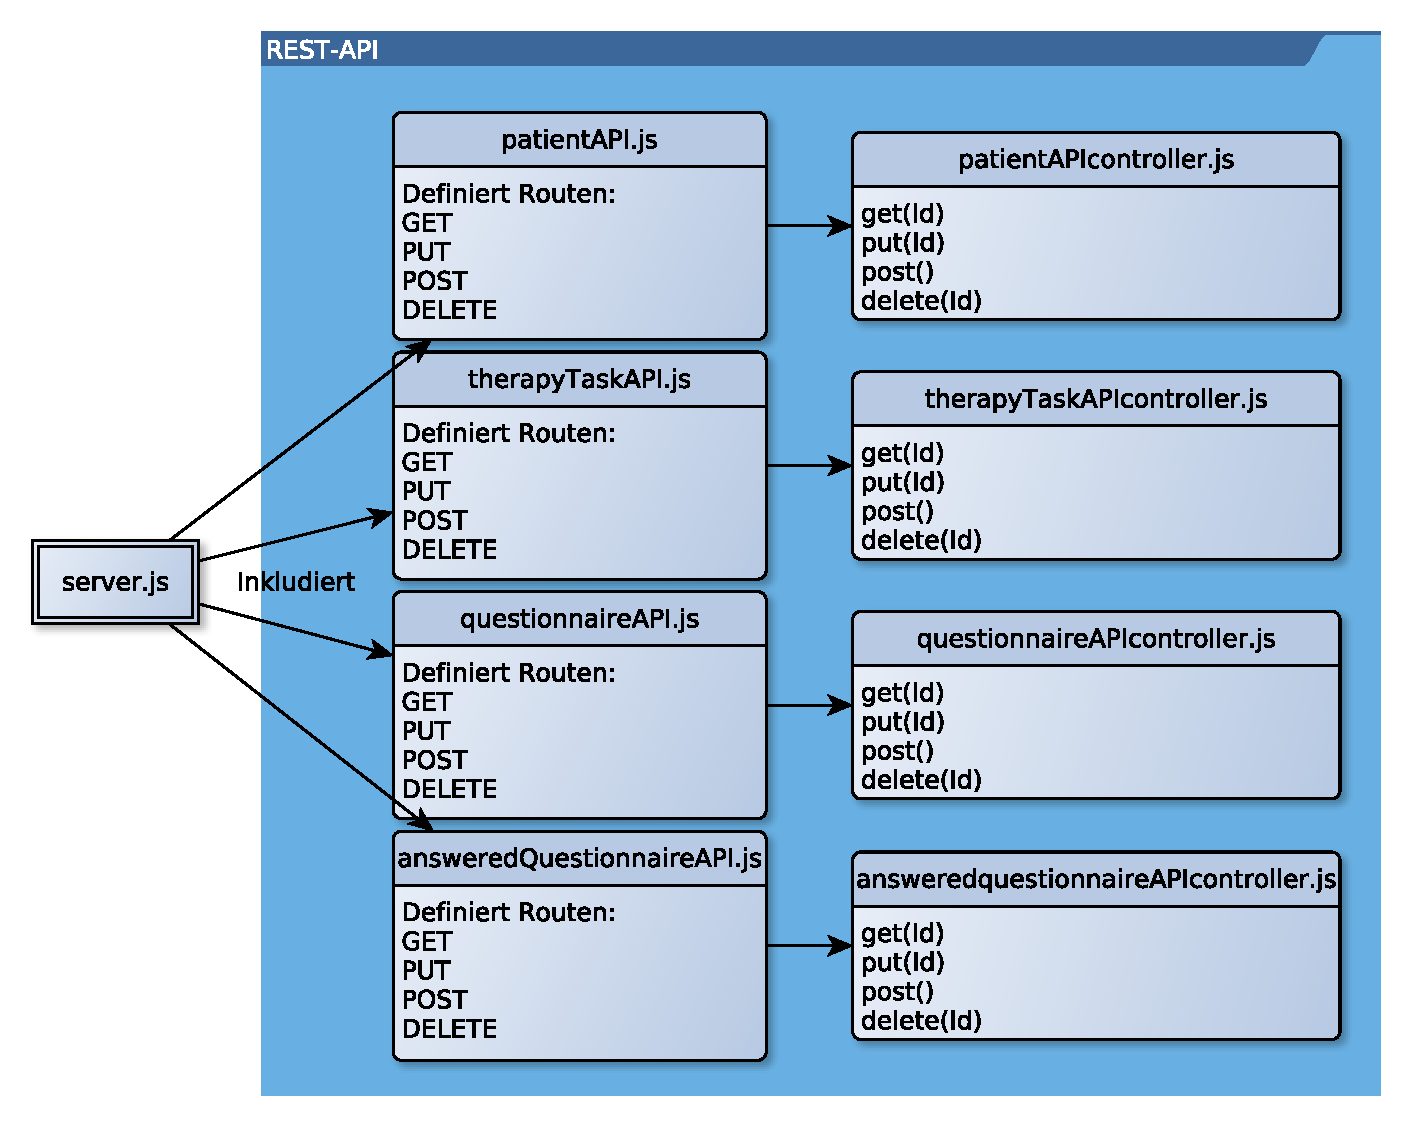
\includegraphics[scale=0.64]{images/RESTAPI_Architektur}
 	\caption[Architektur der REST-API]{Architektur der REST-API}
 	\label{REST Architektur}
 \end{figure}
Durch das \textbf{npm} Paket \textbf{mongoose} \cite{MONGOO16} wird eine Verbindung zu einer auf dem Server laufenden MongoDB Datenbank hergestellt. In dieser werden die Daten zu den Patienten, Aufgaben/Übungen und Fragebögen gespeichert. \textbf{Mongoose} wurden dann die in Abbildung \ref{Datenmodell} gezeigten Modelle der Klassen bekannt gemacht. Hierzu wurden Schemas zu dem Klassen definiert und unter eines einzigartigen Namen den mongoose Modellen mittels \textbf{mongoose.model("<Modell Name"<,"<Schema Objekt">)} hinzugefügt. Nun kann mittels \textbf{Patient.load("<ID">,function())} ein Patient mittels seiner ID aus der Datenbank geladen werden. Anschließen wurden Routen zum Aufrufen aller Patienten und zum speichern, ändern und löschen einzelner implementiert. Für die Web-APIs der therapeutischen Aufgaben, Fragebögen (Muster und beantwortete) wurde die Routen und Schemas analog erstellt.

\newpage
\section{Therapeuten Client} \label{_ImpTherapeutenClient} 
Eine weitere Route wurde eingerichtet, unter welcher sich der Nutzer, in diesem Fall der Therapeut, eine sogenannte \textbf{Single Page Application} in Form einer HTML und damit verbundene JS und CSS Dateien herunter lädt. Diese beinhalten die komplette Logik und Formatierung der Anwendung. Sie basiert auf dem AngularJS Framework und wird mittels HTML5 CSS(Cascading Style Sheets) und JavaScript implementiert. Durch AngularJS bekommt man eine komplett lauffähiges Grundgerüst einer Single Page Application wie in Abbildung \ref{TherapeutenClientSeitenUebersicht} veranschaulicht.

\begin{figure}[H]
	\centering
	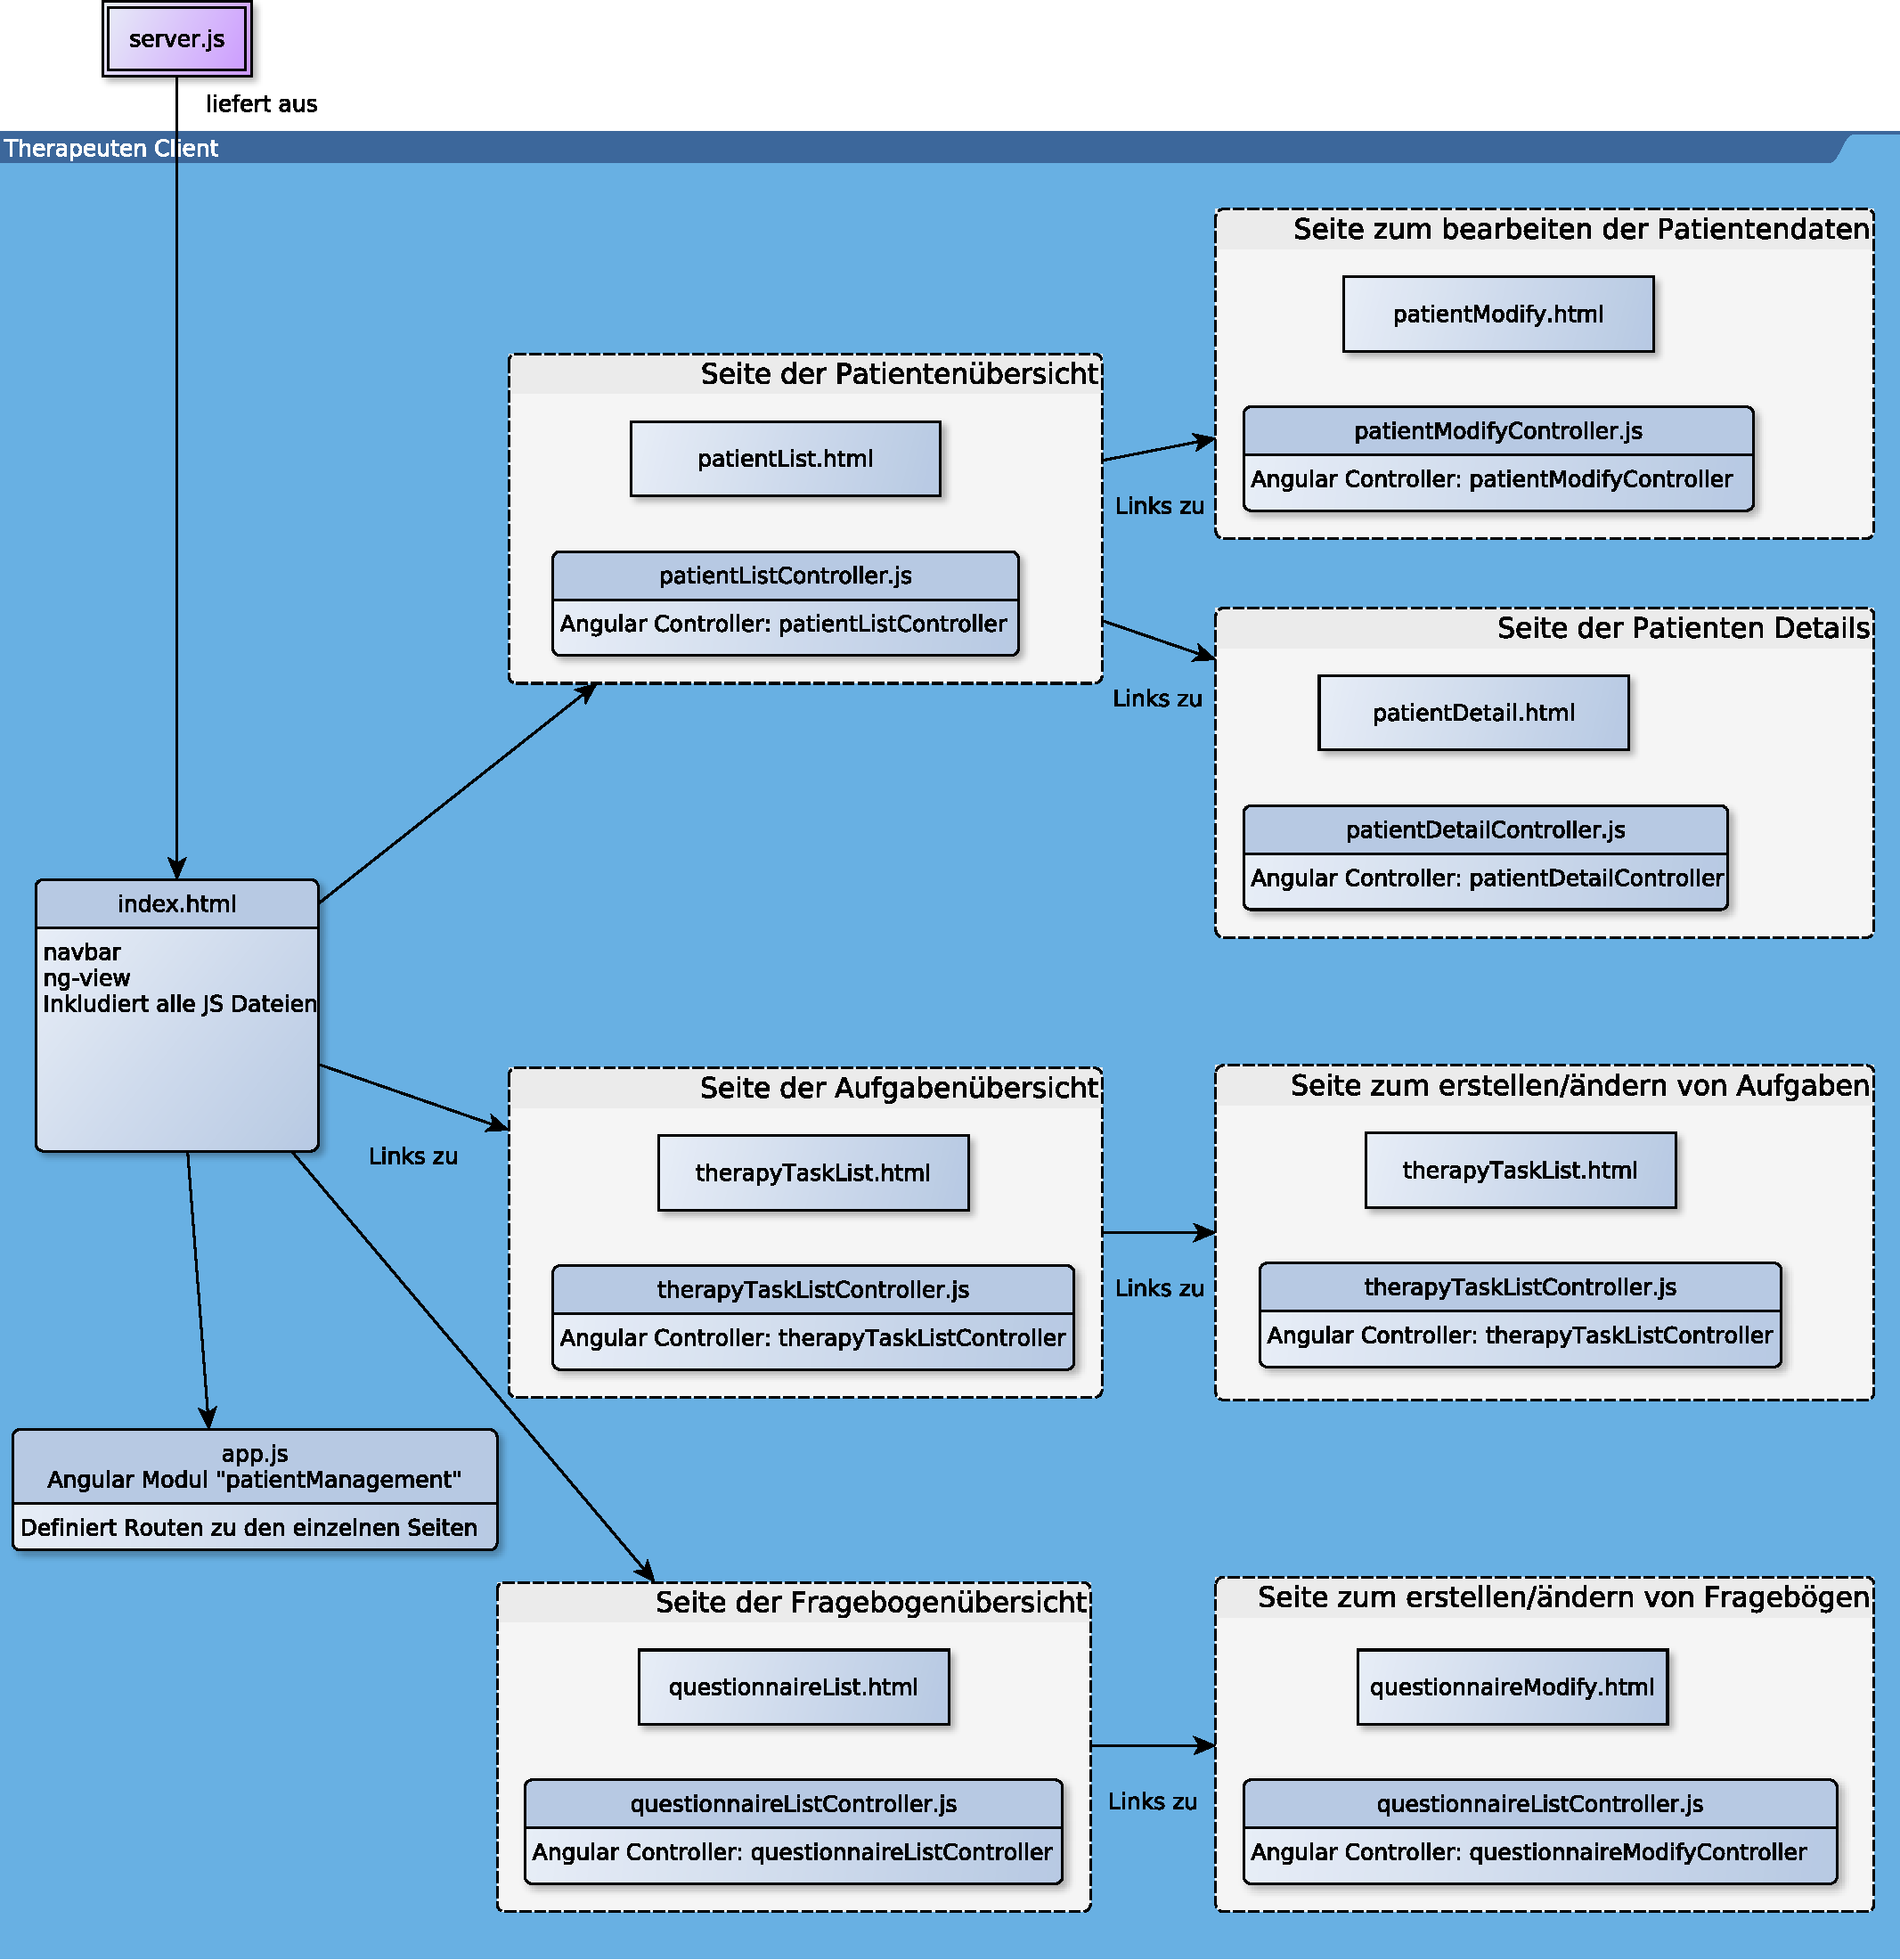
\includegraphics[scale=0.4]{images/TherapeutenClientSeitenUebersicht}
	\caption[Übersicht über die Seiten des Therapeuten Clients]{Übersicht über die Seiten des Therapeuten Clients}
	\label{TherapeutenClientSeitenUebersicht}
\end{figure}

Durch die Verwendung von \textbf{Twitter Bootstrap} wird der Browserapplikation eine Endgerät abhängige Darstellung hinzugefügt. Das bedeutet, dass die Applikation der Größe des Displays, welches sie anzeigt, angepasst wird. Bei kleineren Geräten wird unter anderem die Navigationsleiste in ein SideMenue verschoben, welches auf/-zugeklappt werden kann. Um die horizontal liegende Navigationsleiste auf kleinen Geräten darstellen zu können. Hierdurch wird auch das Gefühl einer klassischen App auf Handy und Tablet gegeben. 
\textbf{Bootstrap} bietet auf seiner Internetseite einfach Beispiele an. Diese wurden verwendet, um eine erste Grundstruktur des Designs der Applikation zu bekommen.

In der \textbf{index.html} werden die benötigten CSS Dateien von AngularJS und Bootstrap geladen. Diese Spezifizieren das Aussehen der geläufigsten HTML Elemente. Zusätzlich werden die benötigten JavaScript Dateien der Angular App und der verwendeten Module eingebunden. Anschließend wird der Grundaufbau der Applikation spezifiziert. Diese besteht aus einer Navigationsleiste mit Links zu den verschiedenen Seiten der Anwendung und einem Container in welchem die sogenannte \textbf{ng-view} verankert ist.  In dieser View wird Angular alle aufgerufenen Seiten anzeigen.

Im \textbf{body} Element wird das Wurzelelement der Angular App \textbf{ng-app="patientManagement"} angegeben. Dieses Angular Modul wird in der \textbf{app.js} mittels \\ \textbf{var app = angular.module("patientManagement", ["<Abhängigkeiten">])} erzeugt. Anschließend wird der \textbf{config} Routine dieses Moduls eine Funktion hinzugefügt, in welcher dem \textbf{routerProvider} die einzelnen Route der Seite mittels \textbf{routeProvider.when("/"<URL">", {"<Einstellungen">})} bekannt gemacht werden. Mit Hilfe des Einstellungsobjekts wird die zur Seite gehörende HTML Datei und die JavaScript Datei welche den Controller beinhaltet spezifiziert. Hierdurch ist es möglich der \textbf{View} einen \textbf{Controller} anzuhängen welcher in der angegebenen Datei mittels \textbf{app.controller(''"<Controller Name">'', function ("<Abhängigkeiten">)\{"<Code">\})} angelegt wird. Dieser Code wird vor dem Anzeigen der Seite aufgerufen.

Durch diese Trennung zwischen Model und View in Verbindung mit der Anbindung an die API des Servers entsteht eine Klassische Model-View-Controller Architektur. Diese trennt das Aussehen, die View, von deren Logik, dem Controller.
Hierdurch ist es möglich Seiten wie in Abbildung [\ref{PatientenUebersicht}, \ref{AufgabenUebersicht}, \ref{PatientDetailsAufgaben}] gezeigt, darzustellen.

\begin{figure}[H]
	\centering
	\includegraphics[scale=0.4]{images/Screenshots/AufgabenUebersicht}
	\caption[Übersicht über die Therapeutischen Aufgaben]{Übersicht über die Therapeutischen Aufgaben}
	\label{AufgabenUebersicht}
\end{figure}
Durch den Controller werden im Hintergrund mittels einer \textbf{HTTP Anfrage} die benötigten Daten zu den Patienten etc. über die Web-API vom Server abgerufen. Diese werden dann gegebenenfalls noch verarbeitet und im sogenannten \textbf{Scope} abgelegt, welcher in den oben genannten Abhängigkeiten in den Controller eingebunden sein muss.
Der \textbf{Scope} ist die Verbindung zur \textbf{View} und dient dieser als Datengrundlage. 

Innerhalb der \textbf{View} kann dann iterativ auf die Daten zugegriffen werden um diese anzuzeigen oder Formulare und andere Eingabemethoden zum verändern der Daten anbieten.
Mittels Angular können die Daten anhand einer Art Vorschleife in der gewünschten Form angezeigt werden. Wodurch die Daten nicht vorformatiert werden müssen.
Buttons können mit im Scope abgelegten Funktionen verknüpft werden, womit auf Nutzerinteraktionen reagiert wird.
\begin{figure}[H]
	\centering
	\includegraphics[scale=0.4]{images/Screenshots/PatientenUebersicht}
	\caption[Seite der Patientenübersicht]{Seite der Patientenübersicht}
	\label{PatientenUebersicht}
\end{figure}

\subsubsection{Übersicht der Patienten}\label{_ImpTCPatientUebersicht}
Die in Abbildung \ref{PatientenUebersicht} gezeigte Ansicht bietet eine Übersicht der auf dem Server gespeicherten \textbf{Patienten}. Hierzu wird mittels der \textbf{get}-Methode des \textbf{http} Moduls eine \textbf{asynchroner HTTP request} an der Server gesendet. Im Falle einer positiven Antwort werden die so erhaltenen Daten im Scope abgelegt. Von nun an können diese in der View durch den \textbf{\{\{"<Variable">\}\}} Operator verwendet werden.

Mit Hilfe von \textbf{ng-repeat="patient in patients"} werden diese Daten in einer Tabellenstruktur angezeigt. Durch \textbf{ng-repeat} kann für jedes Patientenobjekt im \textbf{patients} Array die nachstehenden HTTP Elemente zur Anzeige gebracht werden. Mit Hilfe von \\ \textbf{<a href=" \text{/patientDetails/\{\{"<patient.\_id">\}\} "\text{>}}} kann dann innerhalb des \textbf{ng-repeat} beinhaltenden Elements Beispielsweise ein Link erzeugt werden, welcher die ID des jeweiligen Patienten in der URL übergibt. Hierdurch wird der Nutzer zur Detailansicht des Patienten weitergeleitet. Die angehängte ID kann dort dann anhand des \textbf{routeParams} Moduls ausgelesen werden. 

Um das löschen eines Patienten zu implementieren wurde dem Löschbutton eine Funktion mittels \textbf{scope.deletePatient = function("<patient">)\{\}} im Scope hinterlegt. Diese verwendet die \textbf{delete} Methode des \textbf{http} Moduls um eine HTTP \textbf{delete} Anfrage an den Server zu senden. Bei einer erfolgreichen Anfrage wird das zu löschende Patienten Objekt noch lokal aus den bestehenden Objekten entfernt.
\newpage
\subsubsection{Detailansicht zu einem Patienten}\label{_ImpTCPatientDetail}
In dieser Ansicht können dem Patienten die Aufgaben und Fragebögen zugewiesen werden. Wie in Abbildung \ref{PatientDetailsAufgaben} zu sehen, wird hierzu neben der Aufgabe ein Fragebogen und eine Zeitspanne sowie die Wochentage zu denen die Aufgabe zu erledigen ist ausgewählt. Hierzu werden im Controller alle existierenden therapeutischen Aufgaben und Fragebögen vom Server geladen. Sowie das Objekt des durch die ID spezifizierten Patienten.

\begin{figure}[H]
	\centering
	\includegraphics[scale=0.3]{images/Screenshots/PatientDetailsAufgaben}
	\caption[Ansicht der Patientenübersicht im Web Frontend]{Ansicht der Patientenübersicht im Web Frontend}
	\label{PatientDetailsAufgaben}
\end{figure}

Da dieses Objekt nur die IDs der zugewiesenen Therapeutischen Aufgaben beinhaltet wurde dem Scope eine Funktion \textbf{getTaskById("<id">)} hinzugefügt welche den Name einer Aufgabe zur gegebenen ID zurück liefert. Diese wird in der View mittels \textbf{getTaskById("<Task.PatternId">).name} verwendet, um in der Liste der zugewiesenen Aufgabe den Name und nicht die ID einer Aufgabe anzuzeigen.

Um neue Aufgaben hinzufügen zu können, wird im Scope ein Aufgabenobjekt erzeugt, in welches die Eingaben des Nutzers gespeichert werden. Durch \textbf{ng-model} kann ein Eingabefeld mit einer Variable des Scopes verbunden werden. Durch das \textbf{2-way-binding} von Angular haben Veränderungen im Eingabefeld direkten Einfluss auf die Variable und umgekehrt. Somit kann mittels eines Buttons der vom Typ \textbf{dropdown-toggle} ist die Auswahlfelder für die Aufgaben Fragebögen und Wochentage implementiert werden.
Um eine angenehme Eingabemethode für die Zeitpunkte zu bieten wurde das \textbf{bs-timepicker} Modul hinzugefügt und eingebunden.

Der \textbf{Speichern}-Button ruft die im Scope hinterlegte Funktion \textbf{addTherapyTask()} auf. Diese hängt im Falle das alle benötigten Felder gefüllt sind, das oben erwähnte Aufgabenobjekt im Patientenobjekt an die bestehenden therapeutischen Aufgaben an. Anschließend wird das veränderte lokale Patientenobjekt zur Speicherung an den Server geschickt.
Zusätzlich werden auf dieser Seite die vom Patienten bereits beantworteten Fragebögen angezeigt(Abbildung \ref{PatientDetailsFrageboegen}). Auf deren Grundlage der Therapeut die Therapie verwalten und verbessern kann. Um die Übersichtlichkeit zu verbessern wurde der View ein weiteres \textbf{panel} hinzugefügt in welchem diese angezeigt werden. Diesen \textbf{panels} kann durch hinzufügen unterschiedlicher Klassen ein unterschiedliches Aussehen gegeben werden. Sie bestehen aus einem \textbf{panel-heading} und einem \textbf{panel-body} und werden mittels \textbf{ng-repeat} iterativ angezeigt. 

\begin{figure}[H]
	\centering
	\includegraphics[scale=0.3]{images/Screenshots/PatientDetailsFrageboegen}
	\caption[Seite der Patientenübersicht]{Seite der Patientenübersicht}
	\label{PatientDetailsFrageboegen}
\end{figure}

\newpage

\subsubsection{Verwaltung der Therapeutischen Aufgaben / Übungen}\label{_ImpTCAufgaben}

Anhand der Ansicht in Abbildung \ref{AufgabenUebersicht} hat der Therapeut eine Übersicht über alle bereits angelegten therapeutischen Aufgaben/Übungen. Da die Implementierung dieser Übersichtsseite die selbe ist wie die der Patientenübersichtsseite wird auf diese nicht weiter eingegangen. Durch das Hinzufügen einer neuen Aufgabe kann diese, wie in \ref{TherapeutischeAufgabeDetail} gezeigt, durch \textbf{Name, Beschreibung und beliebigen Materialien} spezifiziert werden. Angehängte Materialien werden mittels \textbf{URLs} angegeben. Anhand derer können eine Vielzahl von Aufgaben gestellt oder unterstützt werden. Beispielsweise durch Videos, GPS Koordinaten, anderen Apps, Bilderserie, oder Texten.

Um diese Daten entgegen nehmen zu können wurde eine Seite erzeugt, welche sowohl zum Anlegen so wie zum Editieren einer Aufgabe dient. Einziger Unterschied der beiden ist, dass beim Editieren einer Aufgabe deren \textbf{ID} beim Seitenaufruf übergeben wird. Ist dies der Fall wird das Objekt der Aufgabe vom Server geladen und mit dessen Daten das Formular gefüllt, das zum ändern der Daten implementiert wurde. Wird keine ID beim Aufruf der Seite mitgegeben, wird ein neues Aufgabenobjekt erzeugt.

Dieses Formular zur Veränderung der Daten wird wie in HTML5 gewohnt mittels eines \textbf{form} Elements eingeleitet. Durch Angular ist es mit Hilfe von \textbf{ng-submit=’’\text{saveTherapyTask()’’}} möglich die angegebene Funktion beim Absenden des Formulars aufzurufen. Diese Funktion entscheidet dann anhand daran, ob eine ID beim Aufruf der Seite mitgegeben wurde ob eine neue Aufgabe mittels eines HTTP \textbf{posts} angelegt oder eine existierende durch einen HTTP \textbf{put} verändert werden muss.

\begin{figure}[H]
	\centering
	\includegraphics[scale=0.25]{images/Screenshots/TherapeutischeAufgabeDetail}
	\caption[Formular zum Editieren oder Erstellen von Therapeutischen Aufgaben]{Formular zum Editieren oder Erstellen von therapeutischen Aufgaben}
	\label{TherapeutischeAufgabeDetail}
\end{figure}

\newpage
\subsubsection{Verwaltung der Fragebögen}\label{_ImpTCFragebogen}
\begin{figure}
	\centering
	\includegraphics[scale=0.4]{images/Screenshots/FragebogenUebersicht}
	\caption[Übersicht über die Fragebögen]{Übersicht über die Fragebögen}
	\label{FragebogenUebersicht}
\end{figure}
Auch für die Verwaltung der Fragebögen wurde eine eigenen Seite eingerichtet. Diese bietet das löschen und editieren der Fragebögen. Es gibt einige gute Node Module, welche eine fertige Oberfläche zum Editieren von Fragebögen zur Verfügung zu stellen.

Jedoch haben alle das Problem , dass es mit diesen nicht möglich ist, Fragen abhängig von der Antwort des Patienten zu machen. Um diese Problematik zu umgehen, wurde ein Tool in die Anwendung eingebaut, dass eigentlich zum modellieren von Business Prozessen verwendet wird und auf der \textbf{B}usiness \textbf{P}rocess \textbf{M}odel and \textbf{N}otation beruht. Dieses Tool von BPMN.io (Camunda BPM) kann völlig auf die eigenen Bedürfnisse zugeschnitten werden. Es is möglich alle Elemente zu verändern. Somit wäre die Möglichkeit gegeben, im Zuge einer finalen Implementierung der Anwendung dem Fragebogeneditor das Aussehen des BPMN Editors zu nehmen. Im Umfang der konzeptionellen Implementierung wurde hierauf jedoch verzichtet.

Die Seite zum Erstellen und Editieren der Fragebögen besteht somit aus dem BPMN Editor und einer Funktion zum Speichern des modellierten Fragebogens. Um den Editor anzeigen zu können wurde der View ein \textbf{<div>} Element mit der ID canvas hinzugefügt. Im mit der View verbundenen Controller wird wiederum geschaut, ob die ID eines Fragebogens beim Aufruf der Seite mitgegeben wurde. Ist dies der Fall wird diese vom Server geladen.

Anschließend wird eine Instanz des eingebundenen Moduls \textbf{BPMNModeler} erzeugt. Diesem wird der bestehende Fragebogen in XML-Form mitgegeben sowie die ID des \textbf{<div>} Elements als \textbf{container} spezifiziert. Innerhalb dieses Elements wird fortan der Editor angezeigt.

\begin{table}[H]
	\begin{center}
		\begin{tabular}{p{4cm} p{10cm}}
		\rowcolor{black!20} \textbf{Type} &  \textbf{Beschreibung} \\ \toprule
		\textbf{single}		& Der Patient kann \textbf{genau eine} Antwort auswählen  \\ \hline \addlinespace
		\textbf{multi}		& Der Patient kann \textbf{mehrere} Antworten auswählen   \\ \hline \addlinespace
		\textbf{text}		& Zu jeder Frage kann ein \textbf{freier Text} geschrieben werden  \\ \hline \addlinespace
		\textbf{rating}		& Mittels Slidern können \textbf{Bewertungen} abgegeben werden                                    
		\end{tabular}
	\end{center}
	\caption{Übersicht über die Typen der Fragen}
	\label{FrageTypen}
\end{table}

Durch das Hinzufügen eines Eigenschaftsfensters zum Editor, können den einzelnen Frage vier verschiedene Typen zugewiesen werden. Diese Typen sind \textbf{single, multi, text und rating} und werden in Tabelle \ref{FrageTypen} näher beschrieben. Dieser wurde beim Erzeugen des Editor Objekts als zusätzliche Option definiert und mit einem weiteren \textbf{<div>} Elements mit der ID \textbf{properties} verknüpft.

\begin{figure}[H]
	\centering
	\includegraphics[scale=0.37]{images/Screenshots/BPMNModeller}
	\caption[Ansicht des BPMN Bearbeitungstool]{Ansicht des BPMN Bearbeitungstool}
	\label{BPMNModeller}
\end{figure}

Mittels des BPMN Editors ist es dann möglich Fragebögen zu gestalten. Fragen werden mittels einem sogenannten Gateway spezifiziert. In dessen Beschreibung kann der Text jener Frage eingetragen werden. Im Eigenschaftsfenster des Gateways kann dann unter Extensions eine neue \textbf{property} mit Namen \textbf{type} hinzugefügt werden. Diese kann die oben erwähnten Typen von Fragen annehmen, welche dem Patienten unterschiedliche Arten der Antwortmöglichkeiten geben. Die einzelnen Antworttexte werden durch sogenannte Tasks spezifiziert und mittels Pfeilen mit dieser verbunden. Die Antworten können dann wiederum mit einer weiteren Frage verbunden werden. Somit kann modelliert werden bei welcher Antwort welche Frage folgt.

Da der BPMN Editor ein Programmteil des Therapeuten Clients ist, welcher auf dem Client des Anwenders läuft aber dennoch Abhängigkeiten zu verschiedenen \textbf{npm} Modulen hat, war es hier nötig das Programm \textbf{browserify} zu verwenden, welches in Abbildung \ref{browserifyErlauterung} veranschaulicht wird. \textbf{browserify} ist ein Kommandozeilentool und nimmt JavaScript Datei entgegen. Es schaut dann welche Abhängigkeiten in dieser Datei mittels \textbf{require} eingebunden sind und erzeugt daraus eine JavaScript Datei welche den gesamten benötigten Code beinhaltet. Hierdurch können auf dem Server installierte Abhängigkeiten auf den Client des Anwenders gebracht und dort ausgeführt werden. 

\begin{figure}[H]
	\centering
	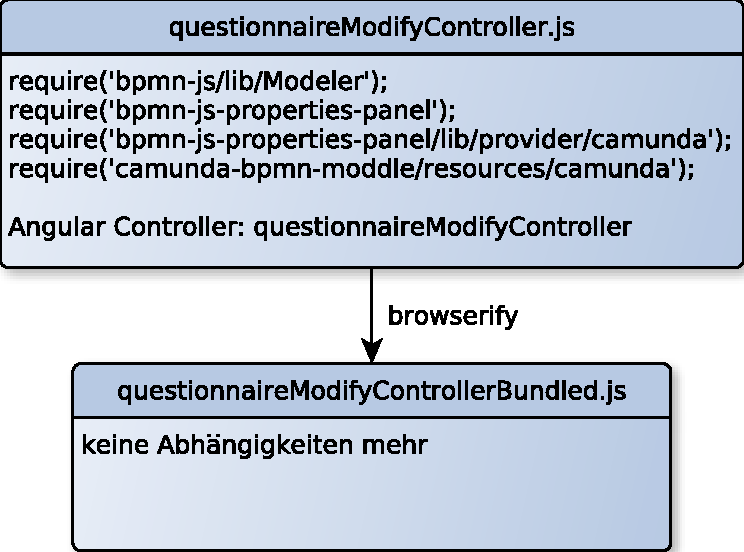
\includegraphics[scale=0.7]{images/browserifyErlauterung}
	\caption[Veranschaulichung von \textbf{browserify}]{Veranschaulichung von \textbf{browserify}}
	\label{browserifyErlauterung}
\end{figure}

\section{Patienten Client}\label{_ImpPatientClient}
Die \textbf{mobile Cross-Plattform-App} wurde auf Grundlage des Ionic Startprojekts \textbf{tabs} implementiert. Dieses Projekt bietet das Grundgerüst einer App mit \textbf{3 Tabs} welche auf jedem Gerät Betriebssystem abhängig angezeigt wird. Diese Web-App [siehe. Kapitel \ref{Hybride Apps}] basiert wie auch der Therapeuten Client auf \textbf{AngularJS}. Im Gegensatz zu diesem wird aber nicht Bootstrap sonder die Ionic eigene Entwicklung für die Oberfläche verwendet. Auf dieser Grundlage entstand die in Abbildung \ref{PatientClient_AufgabenUebersicht} gezeigte Anwendung. Diese bietet einen Tab in welchem der Patient eine Übersicht über die ihm zugeteilten Aufgaben hat mit der Möglichkeit diese im Detail zu betrachten. Sowie einen Tab in dem er sein Profil einsehen kann und einen für die Einstellungen. Jeder dieser Tabs wird durch eine \textbf{HTML Seite} und dem zugehörigen \textbf{Controller} spezifiziert. 

\begin{figure}[H]
	\centering
	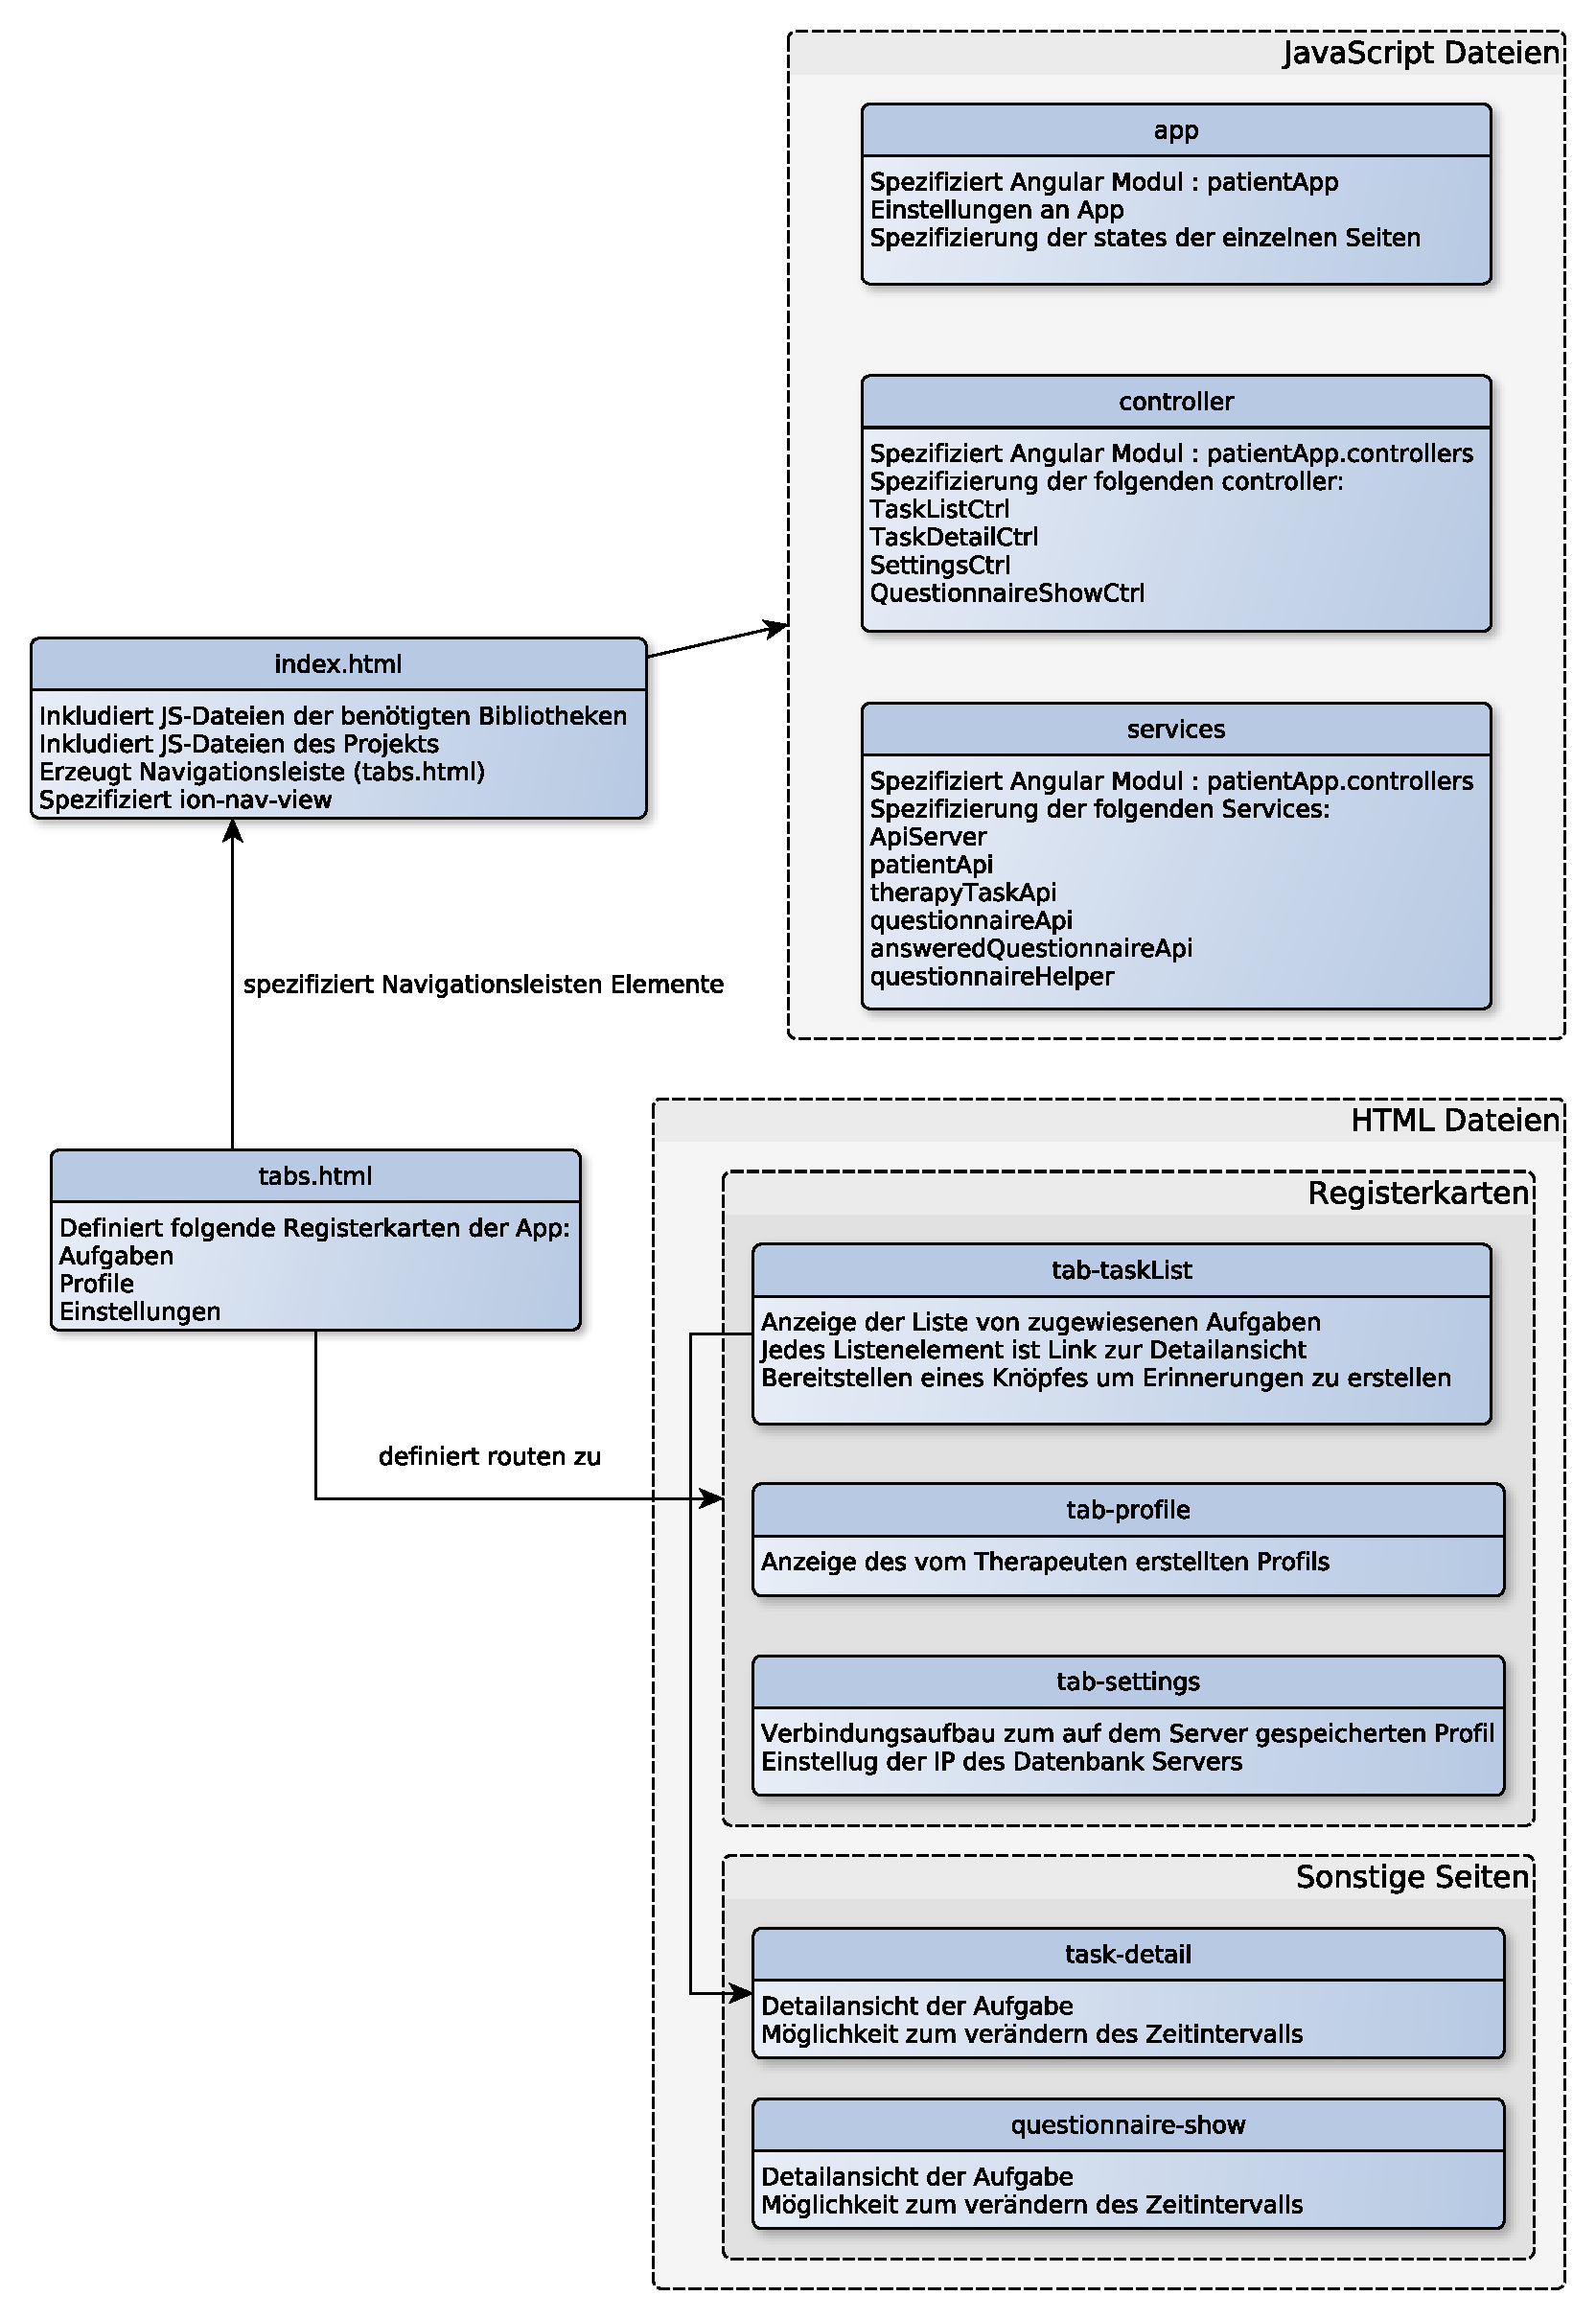
\includegraphics[scale=0.52]{images/PatientenClientArchitektur}
	\caption[Übersicht der Architektur des Patienten Clients]{Übersicht der Architektur des Patienten Clients}
	\label{PatientenClientArchitektur}
\end{figure}

Die HTML Seiten werden im Ordner \textbf{templates} abgelegt. Die JavaScript Dateien sind im Ordner \textbf{js} zu finden. Die App besteht aus \textbf{3 JavaScript Dateien}. Die \textbf{app.js}, \textbf{controller.js} und die  \textbf{services.js} in welcher wiederverwendbarer Code in Form von sogenannten \textbf{factorys} untergebracht werden soll. Diese haben einen Anwendungsweiten eindeutigen Namen und können mit dessen Hilfe in jeden Controller als Abhängigkeit eingebunden und verwendet werden.

Die erste factory (APIServer) wurde erstellt um die Adresse des Datenbankservers System weit an einem zentralen Punkt speichern zu können. Alle Methoden welche mittels HTTP-Anfragen auf den Server zugreifen inkludieren diese factory und lesen aus dieser jene IP Adresse aus.

Um die Server-API von der Anwendung zu abstrahieren, wurde für jede der vier APIs eine eigenen \textbf{factory} angelegt. Diese bieten jeweils eine Funktion zum Abrufen aller vorhanden Einträge sowie das Abrufen eines bestimmten Objekts anhand seiner ID. Mit Hilfe der Funktionen \textbf{remove, create} und \textbf{update} können Einträge auf dem Server angelegt oder unter Verwendung der ID verändert und gelöscht werden. Hierbei wird mit den selben Methoden welche auch schon beim Therapeuten Client verwendet wurden auf den API-Server zugegriffen. Es wurde nur die externe IP Adresse des Servers anstelle der \textbf{localhost} Variable verwendet. Um diese IP einstellbar zu machen wurde für diese ein Eingabefeld im Einstellungstab implementiert. 

Um Daten auf dem Endgerät dauerhaft speichern zu können, wurde der Anwendung das Modul \textbf{ngStorage} hinzugefügt. Diese bietet zum einen den \textbf{sessionStorage} welcher die Daten bis zum schließen der Anwendung behält und den \textbf{localStorage} welcher als persistenter Datenspeicher verwendet wird.

In der \textbf{app.js} wird das Angular Modul \textbf{patientApp} mit seinen Abhängigkeiten spezifiziert. In einer Konfigurationsroutine von diesem Modul wird zu jeder Seite der Applikation ein \textbf{state} im \textbf{stateProvider} angelegt. In jedem \textbf{state} wird spezifiziert unter welcher URL dieser aufgerufen wird, sowie die zugehörige HTML Datei und der Name des Controllers. Hierbei kann ein \textbf{state} einem anderen untergeordnet werden. Dies ist nötig, um Folgeseiten von z.B. Tabs zu definieren.

Um Daten beim Wechsel zu einer anderen Seite übergeben zu können, kann mittels \textbf{/URL/:"<Variablenname">} in einem \textbf{state} definiert werden, dass dieser \textbf{state} für URLs vom Typ \textbf{/URL/"<irgend ein String">} verwendet wird. Mit Hilfe des \textbf{routeParams} Moduls kann dann innerhalb der aufgerufenen Seite auf die übergebenen Daten zugegriffen werden.

Beim ersten Start der Applikation wird der Patient auf den Einstellung Tab geleitet. Hier kann er mittels einer Schaltfläche ein Popup öffnen in welchem er seinen Namen angibt. Wird ein Profil mit diesem Namen auf dem Server gefunden wird dieses Lokal gespeichert. Und die Schaltfläche zum auswählen eines Profils deaktiviert.
Vor dem produktiven Verwenden der App sollte hier ein weiterer Sicherheitsmechanismus eingebaut werden um zu verhindern, dass Unbefugte auf das Profil eines Patienten zugreifen können. 
\subsection{Anzeige der Aufgaben}\label{_ImpPCAufgaben}
Um dem Patienten ein Übersicht über seine zugewiesenen Aufgaben geben zu können wurde die in Abbildung \ref{PatientClient_AufgabenUebersicht} gezeigte Seite eingerichtet. Diese beinhaltet neben der Übersicht über die Aufgaben Buttons zum Erstellen einer Betriebssystem Erinnerungen. 

\begin{figure}[H]
	\centering
	\includegraphics[scale=0.25]{images/Screenshots/PatientClient/AufgabenUebersicht}
	\caption[Ansicht der Aufgaben auf einem Android Smartphone]{Ansicht der Aufgaben auf einem Android Smartphone}
	\label{PatientClient_AufgabenUebersicht}
\end{figure}

Hierzu wurde eine Controller Namens \textbf{TaskListCtrl} erstellt und zusammen mit der \textbf{tab-taskList.html} in den Router eingetragen. Im Controller werden dann die Daten zum Patienten und den existierenden Aufgaben Vorlagen über die oben erwähnten Services vom Server geladen, sofern diese nicht schon lokal vorhanden sind.

In der View wird dann wieder mittels \textbf{ng-repeat} über die im Patienten Objekt vorhandenen Aufgaben iteriert. Jeder so erzeugt \textbf{list-card-devider} Item beinhaltet das HTML-Tag \textbf{ui-sref="tab.task-detail(\{taskId : \$index\})\"}. Hierdurch werden die einzelnen Listenelemente zu Link, welche zur Detailansicht der jeweiligen Aufgabe führen. \textbf{tab.task-detail} ist hierbei der im Router spezifizierte Name der Detailseite. Mittels \textbf{(\{taskId : \$index\})} wird dem Controller der Index der ausgewählten Aufgabe übergeben.
\textbf{\$index} ist eine von \textbf{ng-repeat} bereitgestellte Variable.

Da im Patienten Objekt nur die ID der zugewiesenen Aufgaben gespeichert sind wurde die in Algorithmus \ref{TaskbyId} gezeigte Funktion implementiert. Diese iteriert über die vorhandenen Aufgaben und gibt das passenden Objekt zur ID zurück. Diese Funktion wird wiederum in der View mittels \textbf{\{\{getTaskById(task.PatternId)[0].name\}\}} verwendet.

\begin{lstlisting}[caption={Funktion welche den Namen einer Aufgabe abhängig von der Id zurückliefert},label=TaskbyId]
$scope.getTaskById = function (TaskId) {
	return $.grep(therapyTaskApi.all(false), function (e, x) {
	return e._id == TaskId; 
}); };
\end{lstlisting}
Um die Betriebssystemerinnerungen zu den Aufgaben zu Erstellen wurden Funktionen erstellt, welche mit den Buttons in der View verbunden sind.

\subsubsection{Erstellen von Betriebssystem Erinnerungen}\label{_ImpPCErinnerungen}
Da im Patienten Objekt nur die Wochentage gespeichert sind zu denen die Aufgabe erledigt werden soll, ist noch nicht spezifiziert welches Datum diese Tage haben. Dies wird jedoch benötigt um die Betriebssystem Erinnerungen zu erstellen.

Innerhalb der Oben erwähnten Funktion zur Erstellung der Erinnerungen wird zuerst eine \textbf{Date}-Objekt durch den Standard Constructor erstellt. Das so erzeugte Objekt beinhaltet die Informationen zur momentanen Zeit.

Im \textbf{Date-Objekt} werden die Wochentage als Zahlen zwischen 0 und 6 gespeichert. Wobei die 0 den Sonntag repräsentiert.
Um die Daten der Aufgabenzeitpunkte zu berechnen, wird die rechnerische Distanz zwischen dem Wochentag des Heute-Objekts und den TODO-Wochentagen berechnet.
Diese Distanz wird dann auf das Datum des Heute-Objekts addiert. Durch die Verwendung der \textbf{setDate} Methode kümmert sich das Objekt selbst darum, wenn gegebenenfalls ein Monatswechsel oder ähnliches besteht.

Anschließend werden mittels des \textbf{Cordova Local-Notification Plugins} \cite{CLN16} die einzelnen Erinnerungen erstellt. Das Erinnerungsobjekt muss, wie in Algorithmus \ref{NotificationAdd} beispielhaft dargestellt, verschiedene Eigenschaften beinhalten. Eine \textbf{ID}, hier wird eine laufende Nummer verwendet. Unter \textbf{at} wird das Datum der Erinnerung angegeben.
Als \textbf{title} wird der Name der Aufgabe verwendet.

\begin{lstlisting}[float=htbp, caption={Beispiel einer Funktion zum hinzufügen einer Betriebssystemerinnerung},label=NotificationAdd]
$scope.addSoonNotification = function () {
	var soonDate = new Date();
	soonDate.setSeconds(soonDate.getSeconds() + 15);
	cordova.plugins.notification.local.schedule({
		id: 1987,
		title: "Titel der Erinnerung",
		text: "Klick mich!",
		at: soonDate,
		data: {
		QuestionnaireId: "57e795d2db97f7bd0ee6564a"
	}
	});
};
\end{lstlisting}

Zusätzlich kann der Erinnerung  ein \textbf{data} Objekt angehängt werden. In diesem können beliebige Daten gespeichert werden. Dies wird verwendet um die IDs der Aufgabenvorlage und des Fragebogens zu speichern. 

Mittels \textbf{\$rootScope.\$on(''\$cordovaLocalNotification:click'',function ("<event">, "<notification">, "<state">) \{\}} kann auf den Klick des Nutzers auf die Erinnerung reagiert werden. Es wird dann je nachdem ob es der Beginn oder das Ende des gegebenen Zeitintervalls ist, entweder die Aufgabenbeschreibung oder der zugehörige Fragebogen angezeigt.

Hierzu wird mittels des \textbf{StateProviders} zu eine der Seiten gesprungen und die ID des aufzurufenden Objekts übergeben.
\newpage
\subsubsection{Aufgabendetails einsehen und bearbeiten}\label{_ImpPCAufgabenDetail}
Um die Details zu einer Aufgabe einsehen zu können, wurde eine View \textbf{task-detail} mit dem zugehörigen Controller \textbf{TaskDetailCtrl} erstellt. Mittels der Route \textbf{tab.task-detail} kann auf diese zugegriffen werden. Diese Route übergibt die in der URL angefügten Daten unter der Variable \textbf{taskId}. Diese ID gibt den Index der Aufgabe im Array des Patienten Objekts an. Hierdurch kann beim Aufruf der Seite spezifiziert werden, welche Aufgabe zur Anzeige gebracht wird.

\begin{figure}[H]
	\centering
	\includegraphics[scale=0.25]{images/Screenshots/PatientClient/Aufgabendetails}
	\caption[Name, Erläuterung und angehängte Materialien einer Therapeutischen Aufgabe]{Name, Erläuterung und angehängte Materialien einer Therapeutischen Aufgabe}
	\label{PatientClient_Aufgabendetails}
\end{figure}
Der Controller lädt das Patientenobjekt und die angegebene Aufgabe. Über die gespeicherte ID der Aufgabevorlage wird diese anschließend vom Server abgerufen. Hierdurch ist sichergestellt, dass der Nutzer die \textbf{aktuelle Version} der Aufgabe angezeigt bekommt. Somit ist gewährleistet, dass der Therapeut jederzeit Änderungen an den Aufgaben vornehmen kann und diese auf dem Endgerät des Patienten immer aktuell sind. 

Diese Informationen werden dann wir in Abbildung \ref{PatientClient_Aufgabendetails} gezeigt, angezeigt. Neben dem Titel der Aufgabe wird die Beschreibung und die angehängten Materialien angezeigt. Zum Anzeigen der hinter der \textbf{URL} spezifizierten Informationen wurde eine In-App-Browser in die Anwendung eingebunden. Somit muss der Patient nicht in den Betriebssystem Browser wechseln um die Materialien anzuzeigen.

Um dem Patienten die Möglichkeit zu bieten, das vom Therapeuten vorgeschlagene Zeitintervall zu verändern, wurde die in Abbildung \ref{PatientClient_AufgabendetailsZeit} gezeigten Schaltflächen in diese Seite eingepflegt.
\begin{figure}[H]
	\centering
	\includegraphics[scale=0.25]{images/Screenshots/PatientClient/AufgabendetailsZeit}
	\caption[Übersicht über die Fragebögen]{Übersicht über die Fragebögen}
	\label{PatientClient_AufgabendetailsZeit}
\end{figure}
Da Ionic von Haus aus keinen Funktion zum wählen einer Zeit mitliefert wurde hier das \textbf{ionicTimePicker Plugin} zur Anwendung hinzugefügt. Dieses wird in der \textbf{config}-Phase der App initialisiert. Hier wird der Zeitformat auf 24 Stunden gestellt, sowie die Schrittweite und die Beschriftung der Knöpfe spezifiziert. Durch einen Klick auf die in Abbildung \ref{PatientClient_AufgabendetailsZeit} zu sehende Schaltfläche wird mittels \textbf{ionicTimePicker.openTimePicker()} ein Popup zur Anzeige gebracht in dem der Patient die Möglichkeit hat eine Uhrzeit ohne Datum etc. auszuwählen.

Nach dem Bestätigen der Eingabe werden die neuen Zeitinformationen erst lokal gespeichert. Durch einen Klick auf die Speichernschaltfläche kann das veränderte Patientenobjekt dann zum dauerhaften Speichern an den Server gesendet werden.

\subsection{Anzeige der Fragebögen}\label{_ImpPCFragebogen}
Um dem Patienten die Möglichkeit zu geben, die gestellten Fragebögen zu beantworten wurde eine Seite entwickelt, die ihr Aussehen nach dem Typ der Aufgabe angleicht. In der View \textbf{questionnaire-show} sind die HTML-Elemente für alle vier (in Tabelle \ref{FrageTypen} beschriebenen) Fragetypen vorhanden. Diese sind jedoch durch die \textbf{ng-hide} Direktive, die durch AngularJS angeboten wird, ausgeblendet. Diese Direktiven sind mit im Scope abgelegten Bool Variablen verbunden. Hierdurch können die einzelnen Elemente durch im Controller abgelegten Code angezeigt oder ausgeblendet werden. Ist die zugehörige Variable \textbf{wahr} so ist das HTML-Element ausgeblendet. 
Somit variiert das Aussehen der Seite je nach Fragetyp.
\paragraph{Frage vom Typ single}
In Abbildung \ref{PatientClient_Fragebogen_single} ist ein Beispiel zu einer Frage des Typs \textbf{single} auf einem Android Smartphone zu sehen. Hier kann der Nutzer \textbf{nur eine} der gegebenen Antwortmöglichkeiten auswählen. Die nächste Frage ist, je nachdem was der Therapeut spezifiziert hat, abhängig von der gegebenen Antwort.

\begin{figure}[H]
	\centering
	\includegraphics[scale=0.3]{images/Screenshots/PatientClient/Fragebogen_single}
	\caption[Fragebogenseite beim Fragetyp single]{Fragebogenseite beim Fragetyp single}
	\label{PatientClient_Fragebogen_single}
\end{figure}
\newpage 
\paragraph{Frage vom Typ multi}
In der Abbildung \ref{PatientClient_Fragebogen_multi} ist als Beispiel die Seite gezeigt, wenn der Aufgabentyp \textbf{multi} ist. Dieser Typ erlaubt es dem Endanwender \textbf{mehrere} der zur Verfügung stehenden Antworten auszuwählen.

\begin{figure}[H]
	\centering
	\includegraphics[scale=0.3]{images/Screenshots/PatientClient/Fragebogen_multi}
	\caption[Fragebogenseite beim Fragetyp multi]{Fragebogenseite beim Fragetyp multi}
	\label{PatientClient_Fragebogen_multi}
\end{figure}
\newpage
\paragraph{Frage vom Typ text}
Der in Abbildung \ref{PatientClient_Fragebogen_text} gezeigt Fragentyp gibt dem Anwender die Möglichkeit die Antworten als \textbf{Freitext} zu beantworten. Da das beurteilen von solch einer Antwort den Rahmen dieser Arbeit gesprengt hätte, kann die nächste Frage nicht von der Antwort des Nutzers abhängig gemacht werden.

\begin{figure}[H]
	\centering
	\includegraphics[scale=0.3]{images/Screenshots/PatientClient/Fragebogen_text}
	\caption[Fragebogenseite beim Fragetyp text]{Fragebogenseite beim Fragetyp text}
	\label{PatientClient_Fragebogen_text}
\end{figure}
\newpage
\paragraph{Frage vom Typ rating}
In Abbildung \ref{PatientClient_Fragebogen_rating} ist das Beispiel einer Frage des Typs \textbf{rating} abgebildet. Diese können verwendet werden, wenn der Patient etwas bewerten soll. Die Auswahl resultiert in \textbf{Werten zwischen 0 und 100}.
\begin{figure}[H]
	\centering
	\includegraphics[scale=0.3]{images/Screenshots/PatientClient/Fragebogen_rating}
	\caption[Fragebogenseite beim Fragetyp rating]{Fragebogenseite beim Fragetyp rating}
	\label{PatientClient_Fragebogen_rating}
\end{figure}


Die Route zu dieser Seite stellt in dieser Anwendung eine Besonderheit dar, da sie es zulässt mehrere Variablen in der URL zu übergeben. Neben der ID des Fragebogens kann zusätzlich die ID der anzuzeigenden Frage in der Variable \textbf{questionId} übergeben werden. 

In dem der View zugehörigen Controller \textbf{QuestionnaireShowCtrl} wird das Fragebogen Objekt anhand der übergebenen ID über den oben erwähnten Service vom Server geladen. Anschließend wird der im XML-Format gespeicherte Fragebogen mit Hilfe des \textbf{xml2json-Parsers} \cite{XML2JSON16} in ein JavaScript Objekt geparst. Dies erleichtert den Zugriff auf die einzelnen Objekte erheblich.

Um den Umgang mit einem Fragebogen weiter zu vereinfachen wurde eine weiterer Service Namens \textbf{questionnaireHelper} implementiert.
Dieser bietet verschiedenen Methoden:
\begin{description}
	\item[getStart]\hfill \\
	Welche das Startobjekt zurückliefert 
	\item[getNextQuestionObj]\hfill \\
	Diese Methode erwartet ein Antwort Objekt und liefert die auf diese folgende Frage zurück 
	\item[getQuestionType]\hfill \\
	Liefert den Typ einer Frage zurück 
	\item[getPossibleAnswers]\hfill \\
	Gibt die möglichen Antworten zu einer Frage als Array zurück 
	\item[getQuestionObjById]\hfill \\
	Gibt das Objekt einer Frage anhand derer ID zurück 
	\item[getAnswerObjById]\hfill \\
	Gibt das Objekt einer Antwort anhand derer ID zurück 
\end{description}

Wird nun diese Seite aufgerufen, wird zuerst mittels \textbf{if (typeof \$stateParams.questionId == "\text{undefined}")} geschaut, ob unter der Variable \textbf{questionId} eine bestimmte Frage spezifiziert wurde. Ist dies der Fall wird dieses mit Hilfe der Methode \textbf{getQuestionObjById} aus dem Fragebogen Objekt extrahiert und als aktuelle Frage verwendet. Im Fall, dass keine Frage spezifiziert ist, wird das Start Objekt gesucht und von diesem aus die nächste Frage als aktuelle Frage gewählt.

Anschließend werden anhand der Scope Variablen zuerst alle Fragen HTML-Elemente ausgeblendet. Mittels der Methode \textbf{getQuestionType} wird dann der Typ der Frage ermittelt und das jeweilige HTML-Element wieder aktiviert.
 
Um die Antwort des Nutzers entgegen nehmen zu können wird ein zum Fragentyp passendens Antwortsobjekt erstellt. Dies beinhaltet in jedem Fall den Typ der Frage, um ein späteres Uuswerten und Anzeigen einfach zu machen.

Ist die Frage vom Typ  \textbf{single} wird in diesem Objekt die Frage und die gegebene Antwort gespeichert. Hier wurde auf eine Verbindung zum Fragebogen verzichtet um zu verhindern, dass sich dieser verändert und die gegebene Antwort dann nicht mehr zur eigentlich gestellten Frage passt.

Bei einer Frage vom Typ \textbf{multi} wird für jede Antwortmöglichkeit ein eigenes Antwortenobjekt erzeugt. Jedes dieser Objekte beinhaltet die Variable \textbf{checked}, in welcher festgehalten wird, ob die jeweilige Antwort ausgewählt wurde.

Im Fall das die Frage vom Typ \textbf{rating} ist, wird wiederum für jede Frage ein eigenenes Antwortobjekt erzeugt. Dieses beinhaltet neben den schon erwähnten Variablen eine weitere Namens \textbf{value}. In welchen der Wert der angezeigten Schieberegler gespeichert wird.

Beim Fragetyp \textbf{text} wird auch für jede gestellte Frage ein eigenes Antwortenobjekt erzeugt welches eine Variable \textbf{answerText} beinhaltet mit welcher das Texteingabefeld verbunden ist.

Am Ende der Seite ist eine Schaltfläche eingebaut, welche mit der Funktion \textbf{goToNextSite} verbunden ist.
Diese Funktion schaut nun bei Fragen des Typs \textbf{single} und \textbf{multi} welche der Antworten ausgewählt wurde und ermittelt mittels der Funktion \textbf{getNextQuestionObj} welche Frage als nächstes kommt. Wenn es noch eine weitere Frage gibt wird mittels \textbf{\$state.go("questionnaire-show",\{questionnaireId: qId, questionId: nextQuestion.Id\})} die selbe Seite noch einmal aufgerufen, jedoch mit einer anderen questionId wie zuvor.
Dies wird wiederholt, bis es keine weitere ausgehende Frage zur Antwort mehr gibt und somit das Ende des Fragebogens erreicht ist.




\chapter{Anforderungsabgleich} \label{Anforderungsabgleich} \todo{Anforderungstabellen mit erwähnen, wo kommen die Anforderungen her}
Im folgenden Kapitel wird ein Anforderungsabgleich vorgenommen, dieser gibt Aufschluss darüber welcher der in Kapitel Anforderungsanalyse \ref{Anforderungsanalyse} spezifizierten Anforderungen schlussendlich implementiert wurden.
Hierbei wird im einzelnen auf die jeweiligen Anforderungen, ob nun Funktional oder nicht-funktional, eingegangen und Querverweise in das Kapitel Implementierung \ref{_Implementierung} hergestellt.

\section{Datenbank Server}
\paragraph{Anforderung 1.1 - Datenpersistenz}
Wie in Kapitel \ref{_ImpDatenbankServer} beschreiben, \textbf{wurde} die Datenpersistenz mittels einer MongoDB Datenbank \textbf{umgesetzt}. Diese legt ihr Daten für den Nutzer nicht sichtbar auf dem Dateisystem ab, wo diese Persistent gespeichert werden.

\paragraph{Anforderung 1.2 - Daten Sicherung}
Dieses Feature wurde \textbf{nicht Implementiert}.

\paragraph{Anforderung 1.3 - Datenschnittstelle}
Wie in Kapitel \ref{_ImpDatenbankServer} beschreiben, wurde mit Hilfe des express Frameworks eine REST-API implementiert welche HTTP anfragen entgegen nimmt. Hierdurch ist es Möglich, Daten aus der Datenbank anzufragen, zu verändern bzw. löschen so wie neue Datensätze anzulegen.


\section{Therapeuten Client}
Die Anforderungen an den Therapeuten Client \textbf{wurden alle erfüllt.}
\paragraph{Anforderung 2.1 - Patientenverwaltung}
Dieses Feature \textbf{wurde Implementiert} indem dem Therapeuten Client wie in Kapitel \ref{_ImpTCPatientUebersicht} beschreiben, eine Seite hinzugefügt wurde auf derer er eine Übersicht über seine Patienten hat. Hier können Patienten auch gelöscht werden - Anforderung 2.1.3.

Zusätzlich wurde wie in Kapitel \ref{_ImpTCPatientDetail} beschreiben eine Seite erzeugt mit welche der Therapeut Patienten anlegen bzw. editieren kann - Anforderungen 2.1.1 und 2.1.2.

\paragraph{Anforderung 2.2 - Aufgabenverwaltung}
Mittels der in Kapitel \ref{_ImpTCAufgaben} beschriebenen Seiten ist es dem Therapeuten möglich die Vorlagen für Aufgaben / Übungen zu verwalten. Wie bei der Patientenverwaltung gibt es eine Übersicht in welcher einzelne Aufgaben ausgewählt oder gelöscht (Anforderung 2.2.3) werden können. Mittels der ebenso in Kapitel \ref{_ImpTCAufgaben} beschriebenen Seite zum anlegen und editieren von Aufgaben werden den Anforderungen 2.2.1 und 2.2.2 abgedeckt.

\paragraph{Anforderung 2.3 - Fragebogenverwaltung}
Wie für die Verwaltung von Patienten und Aufgaben/Übungen wurde auch für die Fragebogenverwaltung eine eigene Seite Implementiert, welche in Kapitel \ref{_ImpTCFragebogen} beschreiben wird. Diese bietet die Möglichkeit Fragebögen zu löschen(Anforderung 2.3.3). Die ebenfalls in Kapitel \ref{_ImpTCFragebogen} beschriebene Seite zum erstellen und editieren von Fragebögen erfüllt die Anforderungen 2.3.1 und 2.3.2.

\section{Aufgaben-/Übungsvorlagen}
Die Anforderungen an die Aufgaben-/Übungsvorlagen wurden, wie in Tabelle \ref{TabelleAnforderungsabgleichVorlagen} beschrieben, Teilweise erfüllt.
A.1 bis A.3 sowie A.6 wurden wie in Kapitel \ref{_ImpTCAufgaben} beschreiben erfüllt. 

\begin{table}[htbp]
	\begin{center}
		\begin{tabular}{p{0,5cm} p{6,5cm} p{7,5cm}}
			\rowcolor{black!20} \textbf{Nr.} & \textbf{Bezeichnung} & \textbf{Erfüllt?} \\ \toprule 
			A.1 & \textbf{Name} & \checkmark \\ \hline \addlinespace
			A.2 & \textbf{Beschreibung} & \checkmark \\ \hline \addlinespace
			A.3 & \textbf{Materialien} & \checkmark \\ \hline \addlinespace
			A.4 & \textbf{Kontrollmechanismen} & X \\ \hline \addlinespace
			A.5 & \textbf{Kategorisierung} & X  \\ \hline \addlinespace
			A.6 & \textbf{Verschiedene Erledigungskontexte} & Es wurde nur der Zeitkontext implementiert \\ \hline \addlinespace
		\end{tabular}
	\end{center}
	\caption[Anforderungen an die Vorlage einer Aufgabe/Übung]{Anforderungen an die Vorlage einer Aufgabe/Übung}
	\label{TabelleAnforderungsabgleichVorlagen}
\end{table}

\section{Fragebögen}
Die in Tabelle \ref{TabelleFunktionaleAnforderungenFragebogen} gezeigten Anforderungen wurden abgesehen von Anforderung B.2 \textbf{erfüllt}. Anforderung B.2 wurde als nicht mehr wichtig erachtet, da der Name ausreicht, um einen Fragebogen zu identifizieren. Durch die grafische Darstellen mittels des in Kapitel \ref{_ImpTCFragebogen} beschrieben Tools zur Erstellung/Bearbeitung von Fragebögen wird das wiederfinden eines bestimmten Fragebogens weiter vereinfacht.

\textbf{Anforderung B.3} wurde erfüllt, indem es mittels des grafischen Tools möglich ist, die Fragen und Antworten nach belieben mit einander zu verbinden. Hierdurch kann der Therapeut frei wählen, welche Frage auf eine gegebene Antwort folgt.

Verschiedene Antwortmöglichkeiten wie in \textbf{Anforderung B.4} gefordert wurden wie in Kapitel \ref{_ImpTCFragebogen} beschreiben mit Hilfe eines Zusatz Panels realisiert. Da dies aber nicht sehr intuitiv ist, sollte hier die Möglichkeit wahrgenommen werden, dass man in dem verwendeten Tool neue Elemente einbauen kann. Hierdurch wäre es Beispielsweise möglich zusätzliche Elemente für die einzelnen Fragetypen zu Verfügung zu stellen. Da in dem Tool auch auf Klicks reagiert werden kann, wäre zur Vereinfachung dieses Vorgangs auch ein Kontextmenue denkbar, in welchem man dem allgemeinen Frageelement einen Typ zuweisen kann.





\chapter{Zusammenfassung und Ausblick} \label{Zusammenfassung und Ausblick}
\subsection{Zusammenfassung}
\subsection{Ausblick}

\appendix
% hier Anhänge einbinden
%\input{chapters/AVerwendungDesModems}

\backmatter

\bibliographystyle{plaindin} % Nummern und alphabetisch sortiert
%\bibliographystyle{alphadin} % Buchstaben und sortiert
%\bibliographystyle{abbrvdin} % Nummern und abgekürzte Namen
%\bibliographystyle{unsrtdin} % Nummern und unsortiert
\addcontentsline{toc}{chapter}{Literaturverzeichnis}
\bibliography{2011_Dipl_utf8}
\nocite{*}
\listoffigures
\listoftables
\clearpage
\thispagestyle{empty}

Name: \fullname \hfill Matrikelnummer: \matnr \vspace{2cm}

\minisec{Erklärung}

Ich erkläre, dass ich die Arbeit selbständig verfasst und keine anderen als die angegebenen Quellen und Hilfsmittel verwendet habe.

Außerdem erkenne ich die Satzung der Universität Ulm zur Sicherung guter wissenschaftlicher Praxis an.\vspace{2cm}

Ulm, den \dotfill

\hspace{10cm} {\footnotesize \fullname}
\end{document}
\grid
